\documentclass[lettersize,journal]{IEEEtran}
\usepackage{amsmath,amsfonts}
\usepackage{algorithmic}
\usepackage{algorithm}
\usepackage{array}
\usepackage[caption=false,font=normalsize,labelfont=sf,textfont=sf]{subfig}
\usepackage{textcomp}
\usepackage{stfloats}
\usepackage{url}
\usepackage{verbatim}
\usepackage{amsmath}
\usepackage{amssymb}
\usepackage{graphicx}
\usepackage{tabularx}
\usepackage{cite}
\usepackage{bbm}
\usepackage{pifont}
\usepackage{makecell}
\newcommand{\cmark}{\ding{51}}%
\newcommand{\xmark}{\ding{55}}%
\usepackage{xcolor}
\newcommand{\red}[1]{\textcolor{red}{#1}}
\newcommand{\ul}[1]{\underline{#1}}
\hyphenation{op-tical net-works semi-conduc-tor IEEE-Xplore}
% updated with editorial comments 8/9/2021

\begin{document}

\title{Stochastic Spectrum Prediction via Diffusion Probabilistic Models and Representation Learning}

\author{Chaoyi He, Arya Menon, Jacdon Green, Linda P.B. Katehi$^*$,
\\ Department of Electrical \& Computer Engineering, 
\\ Texas A\&M University, 
\\ College Station, TX, USA
\\ $^*$Correspondence to: katehi@tamu.edu
% ~\IEEEmembership{Staff,~IEEE,}
        % <-this % stops a space
        
% \thanks{Manuscript received April 19, 2021; revised August 16, 2021.}
}

% The paper headers
% \markboth{Journal of \LaTeX\ Class Files,~Vol.~14, No.~8, August~2021}%
% {Shell \MakeLowercase{\textit{et al.}}: A Sample Article Using IEEEtran.cls for IEEE Journals}

% \IEEEpubid{0000--0000/00\$00.00~\copyright~2021 IEEE}
% Remember, if you use this you must call \IEEEpubidadjcol in the second
% column for its text to clear the IEEEpubid mark.

\maketitle

\begin{abstract}
% Wireless networks are integral to modern communication, but are increasingly challenged by spectrum congestion, leading to jitter, packet loss, latency, connection failures, and signal dropout, all of which degrade the user experience. Addressing spectrum congestion is highly challenging with current tools. Our research introduces a novel deep neural network (DNN) based method for predicting spectrum utilization tailored to various wireless environments. Unlike traditional approaches that predict occupancy for entire spectrum blocks, our method accurately evaluates the status of subspectrum spaces, enabling more efficient spectrum sharing. This granularity allows for the integration of diverse signal types, such as radar or satellite communications, into previously underutilized subchannels within occupied spectrum blocks. Our approach leverages historical waveforms processed through an encoder enhanced by contrastive learning, which includes various wireless environments. Future scenario prediction is realized by a diffusion model with an adjustable denoising step, effectively balancing prediction diversity and accuracy and surpassing the performance of static parameter models. The successful use of this model in different wireless communication environments highlights our model's adaptability and efficiency in spectrum sharing. This research advances the spectrum prediction framework by offering a scalable, detailed solution to optimize wireless network management. Our model supports spectrum prediction across 30 wireless communication environments, maintaining stable performance for 32 future time frames, with an Average Displacement Error (ADE) and Final Displacement Error (FDE) of 0.047, indicating the potential for further extensions. The model's spectrum domain prediction performance is validated by a receiver operating characteristic (ROC) curve, with an area under the ROC curve (AUC) of 0.84, demonstrating its robustness and accuracy.
Wireless networks face increasing spectrum congestion as demand grows, resulting in degraded quality of service including latency, packet loss, and connection failures. Conventional spectrum management treats allocated frequency blocks as monolithic units, leaving sub-block capacity underutilized even when portions are unoccupied. This paper presents a deep neural network framework for predicting spectrum utilization at sub-channel granularity across diverse wireless environments. The system operates on raw time-domain signal waveforms rather than aggregated power measurements, enabling predictions at the resolution of individual OFDM frames (approximately 13~$\mu$s) — significantly finer than prior methods that operate on timescales of seconds to hours. The architecture consists of three stages: (1) an encoder trained via contrastive learning compresses historical waveform data into a compact latent representation that generalizes across environments; (2) a probabilistic diffusion model, conditioned on this representation, generates plausible future time-domain signals; and (3) a convolutional neural network maps the generated signals to frequency-domain occupancy predictions for eight sub-blocks within an 80 MHz band. The diffusion model's stochastic generation process captures the inherent uncertainty in user arrival and departure patterns, modeled as a queuing process. Multiple samples are drawn and aggregated via majority voting to produce robust occupancy forecasts. The framework is validated across 30 simulated wireless environments based on the IEEE 802.11ax standard, predicting 32 future time frames with a normalized Average Displacement Error (ADE) of 0.047 and a system-level ROC AUC of 0.84 for sub-channel occupancy classification. These results suggest that the proposed framework is a promising step toward enabling fine-grained dynamic spectrum sharing, though validation on real-world hardware remains an important direction for future work.
\end{abstract}

\begin{IEEEkeywords}
Spectrum Prediction, Dynamic Prediction, Spectrum Sharing, Wireless Spectrum Allocation
\end{IEEEkeywords}

\section{Introduction}
\IEEEPARstart{W}{ireless} communication has become foundational infrastructure for modern society, supporting everything from cellular networks and WiFi to the rapidly expanding Internet of Things (IoT), autonomous vehicles, and satellite systems. As these diverse technologies proliferate, they compete for a finite resource: radio frequency spectrum. This competition leads to congestion, degraded quality of service, and inefficient utilization of available bandwidth — problems that are only expected to worsen as the number of connected devices continues to grow \cite{intro_ref1, intro_ref2, intro_ref3, intro_ref4}.

% Recent advancements in machine learning, particularly deep learning (DL), have opened new avenues in predictive analytics. Deep Neural Networks (DNNs), renowned for extracting patterns from high-dimensional data, have shown significant potential in various domains, including image recognition, natural language processing, and complex system modeling \cite{intro_ref5, intro_ref6}. However, applying DNNs to spectrum prediction presents unique challenges due to wireless signal data's inherent temporal, spatial, and frequency-related dependencies \cite{intro_ref7, intro_ref8, intro_ref9}.

This paper addresses that inefficiency with a central goal: enabling other devices and signal types — such as radar, satellite links, or IoT sensors — to transmit simultaneously within the same frequency band as WiFi, by precisely identifying and utilizing the subchannels that WiFi is not actively using at any given instant. As illustrated in Fig.~\ref{fig_1}, rather than waiting for an entire WiFi transmission to complete before reallocating spectrum, our approach predicts, frame by frame, which subchannels within an occupied band are actually vacant. This allows secondary users to immediately access those gaps without interfering with the primary WiFi signal, effectively allowing multiple heterogeneous systems to coexist within the same band at the same time.

The practical impacts of this capability are: First, it directly reduces spectrum congestion by converting wasted capacity into usable bandwidth for additional devices. Second, it increases overall spectral efficiency by enabling dense, simultaneous sharing among different signal types — a capability that becomes increasingly critical as wireless demand outpaces the availability of new frequency allocations.

Achieving this requires solving a difficult prediction problem: determining, with high temporal and frequency resolution, which subchannels will be occupied or vacant in the near future. Traditional spectrum sensing methods detect current occupancy but cannot anticipate upcoming changes, such as when a user's transmission is about to end or when a new user is about to begin. Prior machine learning approaches have relied on power measurements or binary occupancy labels to predict spectrum utilization, but typically operate at temporal resolutions of hundreds of milliseconds to minutes \cite{intro_ref1, intro_ref4, intro_ref7, intro_ref8, intro_ref9, intro_ref12, intro_ref13, intro_ref14, intro_ref15, Saad_2016, intro_ref17, intro_ref18, intro_ref19, intro_ref20}, and at frequency granularities of full channels rather than individual sub-carriers. This limits their applicability to real-time, sub-channel-level sharing scenarios.

Our approach overcomes these limitations by operating directly on raw time-domain signal waveforms, which contain the detailed information necessary to capture temporal patterns. The framework combines three components: a contrastive-learning-based encoder that compresses historical waveforms into a compact representation generalizable across wireless environments; a probabilistic diffusion model that generates realistic future signal waveforms conditioned on that history \cite{intro_ref10}; and a convolutional neural network that translates the predicted time-domain signals into frequency-domain occupancy maps at the subchannel level \cite{intro_ref11}. This pipeline produces predictions at the granularity of individual OFDM frames — approximately 13 microseconds — far exceeding the resolution of existing methods.

The system is validated across 30 simulated wireless environments based on the IEEE 802.11ax (WiFi 6) standard. It reliably predicts 32 future time frames with an Average Displacement Error (ADE) and Final Displacement Error (FDE) of 0.047 and achieves an area under the ROC curve (AUC) of 0.84 for spectrum occupancy classification. These results demonstrate that the proposed framework can provide the fine-grained, real-time spectrum awareness needed to support simultaneous multi-system coexistence within shared frequency bands — a key step toward alleviating spectrum congestion in next-generation wireless networks \cite{intro_ref17, intro_ref18, intro_ref19}.



% As illustrated in Figure \ref{fig_1}, traditional communication policies allow certain users to share frequency bands with Orthogonal Frequency-Division Multiplexing (OFDM) modulation. However, any unused spectrum within the allocated block is typically padded, preventing other users from utilizing this available spectrum. This padding policy remains the same in the newest Orthogonal Frequency-Division Multiple Access (OFDMA) modulation, which improves the spectrum efficiency by allowing the user to use part of the block when the system has a lot of users. A new user can only begin transmission once the current data package is fully transmitted. While this policy ensures continuous transmission integrity and synchronization, avoiding catastrophic interference and errors during dynamic spectrum management, it also leads to inefficiencies and increased latency.

% This inefficiency could be more problematic in high-density environments, such as IoT ecosystems and autonomous vehicular communications, where timely and efficient spectrum utilization is critical. Our research addresses this inefficiency by predicting future spectrum conditions, enabling the immediate integration of new users into the communication system. Unlike existing spectrum prediction methods that predict occupancy for entire spectrum bands, our approach assesses sub-channel status within OFDM modulation. This granularity allows for more efficient spectrum sharing, facilitating the integration of diverse signal types, such as radar or satellite communications, into previously underutilized sub-channels within occupied bands. Our model enhances network performance and adaptability in dynamic wireless environments by optimizing resource utilization and supporting diverse signals.

% Previous AI-based spectrum prediction approaches have limitations in dealing with real-time dynamic changes \cite{intro_ref1, intro_ref4, intro_ref7, intro_ref8, intro_ref9, intro_ref12, intro_ref13, intro_ref14, intro_ref15, intro_ref16, intro_ref17, intro_ref18, intro_ref19, intro_ref20}. Without utilizing signal waveforms as input, they fail to model the queueing nature inherent in communication environments. Recurrent Neural Networks (RNNs) and Convolutional Neural Networks (CNNs) are insufficient for capturing the probabilistic characteristics of queue networks. As a result, prior works can only predict spectrum occupancy over intervals of seconds or longer and are unable to effectively anticipate user departures and arrivals. Our approach leverages probabilistic AI models and waveform inputs to overcome these limitations, enabling accurate short- and long-term predictions of user behavior in dynamic spectrum environments.

% This paper introduces a DNN-based spectrum-sharing method designed for diverse wireless environments. Our approach begins with compressing historical signal data through an encoder enhanced by contrastive learning, which feeds into a diffusion model to generate potential future signals. This probabilistic diffusion model captures the distribution of possible future signals, balancing the fidelity and speed of predictions \cite{intro_ref10}. The resulting future signals are then analyzed by a convolutional neural network (CNN) to predict future spectrum conditions \cite{intro_ref11}.

% Our contributions focus on implementing a conditional generative deep neural network model within a communication system, combined with self-supervised representations to compress historical information. This approach enables the neural network to capture and interpret implicit information within the communication environment. Unlike previous works, which primarily focus on spectrum prediction based on signal power and often treat wide frequency bands as a whole or perform predictions at low time domain resolutions (e.g., by minute, hour or day) \cite{intro_ref12, intro_ref13}, our model offers a more granular and dynamic solution, promising a significant advancement for cognitive radio systems.

% First, we introduce a novel framework for spectrum prediction that effectively integrates contrastive learning with generative models. This combination addresses the long-standing challenges of indeterminacy and stochastic properties inherent in wireless signal prediction, a critical issue in the field \cite{intro_ref14, intro_ref15, intro_ref16}. Second, we validate our method's performance across various wireless communication environments through extensive experiments. These tests demonstrate the robustness and adaptability of our approach, setting a new benchmark for spectrum prediction methodologies. Although our research currently focuses on the feasibility of neural networks in this domain, its potential applications could extend across a broad spectrum of scenarios, from urban cellular networks to remote IoT deployments, pending further development and real-world testing.

% Our model can predict the spectrum in 30 wireless communication environments, maintaining stable performance with 32 OFDM time frames. The Average Displacement Error (ADE) and Final Displacement Error (FDE) remain consistent at 0.047, indicating the potential for further extension of the predictions into the future. The model's spectrum domain prediction performance is evaluated using the receiver operating characteristic (ROC) curve, with an area under the ROC curve (AUC) of 0.84.

% This study introduces a novel framework for spectrum prediction by implementing generative AI conditioned on historical information. It provides a practical toolkit to improve the efficiency of current and future wireless networks. By addressing the limitations of traditional spectrum sensing and allocation strategies, our work paves the way for more intelligent, adaptive wireless communication systems capable of meeting the demands of an increasingly connected world \cite{intro_ref17, intro_ref18, intro_ref19}.

\section{Spectrum Prediction: A Historical Perspective and Current State-of-the-Art}\label{sec:lit_review}
The history of spectrum sensing and prediction is closely tied to the development of cognitive radio systems, which aim to improve spectral efficiency, in large part by enabling wireless devices to access empty spectral bands. Early techniques relied on sensing the current spectrum, extracting statistical models of wireless access, and using these models to predict future occupancy. These statistical approaches were eventually succeeded by machine learning and, more recently, deep learning methods, which generally outperform them. The superior performance of deep learning stems from its ability to capture complex non-linear and multidimensional dependencies within the data. However, deep learning-based methods are not always practical for resource-constrained edge applications; consequently, hybrid approaches that combine classical techniques with AI-based methods are sometimes adopted. This section provides an overview of the evolution of spectrum prediction methods by summarizing seminal techniques published over the previous decades. For a detailed literature review on spectrum sensing and prediction, readers are invited to review \cite{Yucek_2009, He_2010, Xing_2013, Chen_2016, Ding_2017, Wang_2024}. Notably, spectrum occupancy can be determined across various domains such as time, frequency, space, code, and angle of arrival \cite{Yucek_2009} and also jointly in time and frequency. This review focuses primarily on predicting spectrum in the time-frequency (temporal-spectral) domain, while also covering methods that enable spatial-temporal-spectral predictions.

Large-scale measurement campaigns have provided valuable insights into spectrum utilization \cite{Chen_2016}. As of 2023, measured spectrum use in urban U.S. LTE/5G bands is strongly band‑ and direction‑dependent: downlink channels have much higher occupancy probabilities than uplink, while CBRS and 5G n77 stand out with significantly lower occupancy than the other cellular bands studied \cite{Raouf_2023}. More importantly, measurement campaigns have reported that while certain spectral bands at specific locations and time durations exhibit high occupancy, large portions of the spectrum are lightly utilized \cite{Wellens_2007, Engiz_2021, Kozlowski_2021}. This observation motivates the need for predicting spectral vacancies to enable more effective utilization. 

Spectrum prediction is closely linked to spectrum sensing, for which a variety of techniques have been developed for both narrowband and wideband situations \cite{Muzaffar_2024}. While many studies use common methods like power level measurements or energy detection, more advanced algorithmic approaches include likelihood testing \cite{Segura_2010}, cyclostationary detection \cite{Yucek_2009}, and wavelet-based sensing \cite{Tian_2006}, among others \cite{Muzaffar_2024}. To identify larger occupancy trends, the concept of average duty cycle is often utilized to get a general picture of available bands; however, this metric is highly sensitive to detection thresholds and measurement location \cite{Wellens_2010}. The reliance on these explicit sensing steps is a key differentiator among prediction methods: classical approaches are highly dependent on them, whereas advanced AI techniques can often perform sensing and prediction directly from the data.

\subsection{Classical Methods for Spectrum Prediction}

Classical spectrum occupancy prediction methods build upon the large-scale measurement campaigns described above and rely on extensive occupancy and evolution modeling \cite{Chen_2016}. Various studies also introduced statistical models, where the temporal evolution of spectrum occupancy is modeled using continuous-time Markov or semi-Markov chains, where spectral bands switch between occupied or unoccupied states through four empirically obtained state transition probabilities. These models explicitly characterize the random sojourn (holding) times in each state through fitted probability distributions. Some models also consider the previous state in time and the adjacent channel state, yielding eight transition probabilities to describe temporal evolution \cite{Gibson_1994, Percival_1997}. In certain channels, discrete time Markov chains might be more appropriate. From a prediction standpoint, the problem is cast as a hidden Markov model (HMM): only noisy observations of current and past channel states are available, while the parameters of an (often non stationary) underlying Markov chain are learned and the hidden occupancy states are inferred \cite{Chen_2011, Akbar_2007}. Conventional HMM approaches typically target one‑step‑ahead prediction and are not designed for accurate multi‑slot prediction horizons. In \cite{Saad_2016}, however, HMM was extended for multi-step predictions by casting it as a maximum-likelihood classification problem. The underlying Markov Chain can also be estimated using Bayesian Inference \cite{Xing_2013_channel_qual} but these models are sensitive to the selection of probability distributions \cite{Pan_2026}.

While Markov models are extremely effective in capturing the temporal evolution of the spectrum, they do not capture the frequency or spatial dimensions or incorporate location information. Linear regression models offer a pathway for incorporating these dimensions into the predictive framework. Building on early time‑series work by Yule on autoregressive (AR) modeling \cite{Yule_1927} and Slutsky on moving‑average (MA) representations \cite{Slutzky1937Summation}, Box and Jenkins \cite{Box_1978} unified these into the autoregressive moving‑average (ARMA) family and later generalized them to the autoregressive integrated moving‑average (ARIMA) class. ARIMA models represent the current value of a (possibly differenced) time series as a linear function of its past values and past shocks, and models are widely used to capture serial correlation and non‑stationarity in forecasting applications across economics, climate, and health. All four models — AR, MA, ARMA, and ARIMA — find usage in wireless spectrum prediction, and mathematical expressions for all four are available in Section III of \cite{Ding_2017}.

The correct autoregressive model is selected by calculating the auto-correlation function (ACF) and partial-autocorrelation function (PACF). Using ARIMA($p, d, q$) as the framework — where $p$ represents the number of autoregressive lag observations, $d$ is the degree of differencing required for stationarity, and $q$ is the size of the moving average window — these functions identify the underlying structure of the wireless spectrum data. Specifically, the spectrum is modeled as AR if the PACF cuts off while the ACF tails off, MA if the ACF cuts off while the PACF tails off, and ARMA if both functions tail off. If the ACF fails to tail off quickly and differencing is applied ($d>0$), ARIMA is appropriate. In terms of real-world applicability, \cite{Hou_2021} showed that the AR model works when predicting busy/idle durations in heavy WLAN traffic, whereas 603.25-843.25 MHz occupancy in Chinese TV bands was best predicted using an MA model \cite{Su_2009}. The ARMA model works well in channels that show cyclic behaviors \cite{Tabassam_2011} and Seasonal ARIMA allowed for effective forecasting of GSM 850 MHz occupancy in Colombia (traffic measured in 2012) \cite{Pedraza_2016}.  

\subsection{Basic Machine Learning Models}

Since 2010, machine learning (ML) and neural networks have gained application in spectrum prediction, with a key advantage being that they do not require prior knowledge of the spectrum occupancy characteristics unlike many classical approaches \cite{Tumuluru_2010}. The simplest ML model that can perform spectrum prediction tasks is the multi-layered perceptron (MLP). Interestingly, \cite{Yin_2011} states that the ARIMA model is essentially a special case of the MLP but demonstrates slightly worse results. When the data input to the MLP is normalized, its generalization and prediction accuracy across frequencies and services improve. MLPs have been shown to be effective in predicting GSM bands \cite{Yin_2011} as well as TV broadcast frequencies \cite{Winston_2013}. Since neural networks require a training period, which can limit flexible updates, some researchers have also examined extreme learning machine (ELM) methods, which offer faster training than the MLP while maintaining prediction accuracy \cite{Yang_2014}. The inclusion of a feedback loop allows cognitive radio systems to use previous predictions as inputs, a technique employed by recurrent neural network-based methods \cite{Taj_2011, Yang_2013}. Other machine learning algorithms like learning automata \cite{Golestanian_2014} and support vector machines (SVM) \cite{Ni_2011} have also been reported for wireless spectrum prediction. SVM guarantees optimal convergence and has a small number of parameters, making it attractive for edge applications compared to the MLP. While these basic AI/ML methods can capture non-linear relationships in spectrum occupancy, they still require some degree of feature engineering or feature extraction. This dependency on manual feature engineering, along with the desire for a fully data-driven approach that can also predict the spectrum across multiple domains, drove the adoption of deep learning and other advanced AI methods.

\subsection{Advanced AI/ML Models and Current State-of-the-Art}

Since the landmark deep-learning work of Krizhevsky, Sutskever, and Hinton in 2012 \cite{Krizhevsky_2012}, deep learning has been applied to many areas, including spectrum prediction \cite{Wang_2024}. Deep learning-based models such as Long Short-Term Memory (LSTM) \cite{Wang_2017, Ozyegen_2020}, and Convolutional Neural Networks (CNN) \cite{Jia_2020} have enabled a data-driven approach for predicting spectral occupancy across spatio-temporal-spectral domains. Of these, techniques like LSTM and Recurrent Neural Networks (RNNs) have largely been restricted to single time-step prediction, whereas CNNs have been demonstrated for multi-step prediction \cite{Yu_2018}. 

Long-term spectrum prediction or multi-step prediction is particularly useful for optimizing spectrum utilization and basic machine learning models can be modified to perform this function. \cite{Wang_2024} classifies such models as seq2seq models, which are typically constructed using RNN, LSTM, and ConvLSTM. For time-frequency prediction, combinations of basic AI/ML models have proven to be successful, including hybrid architectures LSTM-CNN \cite{Zhang_2021_Accurate} and CNN-BiLSTM \cite{Ding_2020_Deep}. Hybrid deep-learning models have also been applied to joint spatial-temporal-spectral domain predictions, as demonstrated in \cite{Shawel_2019, Wen_2023}.
Another area of research is the prediction of spectrum in the presence of sparse or missing data and the deep learning method known as Deep Transfer Learning (DTL) has proven effective \cite{Li_2023}. This technique involves copying the weights from a pretrained spectrum prediction model, freezing early layers to retain general features, and re-initializing the final layer for learning the new, sparse frequency bands. However, because occupancy patterns vary across signal types, researchers use Transfer Component Analysis (TCA) to ensure band similarity before transfer \cite{Li_2023}. Additional optimizations include Data Augmentation to combat sparsity, Knowledge Distillation \cite{Cheng_2023} to compress complex model knowledge into efficient architectures for faster prediction, and Generative Adversarial Networks (GANs) to synthesize missing samples when similar spectral data is available \cite{Lin_2021}. These AI models treat sparse or missing data in the preprocessing step and attempt to fill in this data prior to prediction. In contrast, a technological leap is achieved by designing models with embedded imputation mechanisms where models like GRU-D, LSTM-M, and CBRNN learn the underlying pattern in missing data and simultaneously predict future spectrum evolutions \cite{Wang_2024}.  

The development of the Transformer architecture, introduced by the seminal 'Attention Is All You Need' paper \cite{Vaswani_2017}, has opened new possibilities in spectrum prediction. Unlike techniques like LSTM, Transformers can retain context information across longer time frames and are therefore highly effective at long-term spectrum prediction. In \cite{Pan_2023}, a model titled ‘Autoformer CSA’ applied the self-attention mechanism — the core engine of transformers — to spatial and frequency channel predictions over large time frames (up to 120 mins). \cite{Pan_2025} introduces a Vision Transformer LSTM (ViT-LSTM) model that combines visual self-attention with LSTM to achieve spatiotemporal spectrum prediction. Techniques like Singular Spectrum Analysis (SSA) can also be powerful at decomposing and extracting features from complex spectral evolution datasets; for instance, in \cite{Ben_2025}, SSA was combined with an attention-based directional LSTM for improved spectral prediction. Recent work has explored multi‑scale and hybrid Transformer architectures for spectrum prediction, including models that combine convolutional feature extractors with self‑attention (e.g., MSTFformer \cite{Shuang_Li_2025} and CNN-Transformer \cite{Guan_2025}) and temporal sequence backbones such as DB-LSTM \cite{Xu_2024}, improving long‑horizon forecasting and multi‑resolution pattern modeling compared to conventional RNN‑based approaches.

In summary, the literature has progressed from statistical occupancy models to deep-learning and Transformer-based predictors of steadily increasing accuracy and horizon. Nevertheless, the methods surveyed above share three limitations: they operate on aggregated power measurements or binary occupancy labels rather than on the underlying waveforms, their temporal resolution is coarse (hundreds of milliseconds to minutes), and they do not explicitly model the stochastic arrival and departure of individual users. These limitations motivate the framework developed in this paper — a generative model that operates directly on raw time-domain waveforms to anticipate occupancy transitions at the OFDM-frame level. Section~\ref{sec:data} first describes the IEEE 802.11ax simulation framework used to generate labeled waveform data with realistic multi-user dynamics; Section~\ref{sec:methods} then details the proposed architecture.

\begin{figure*}[!t]
\centering
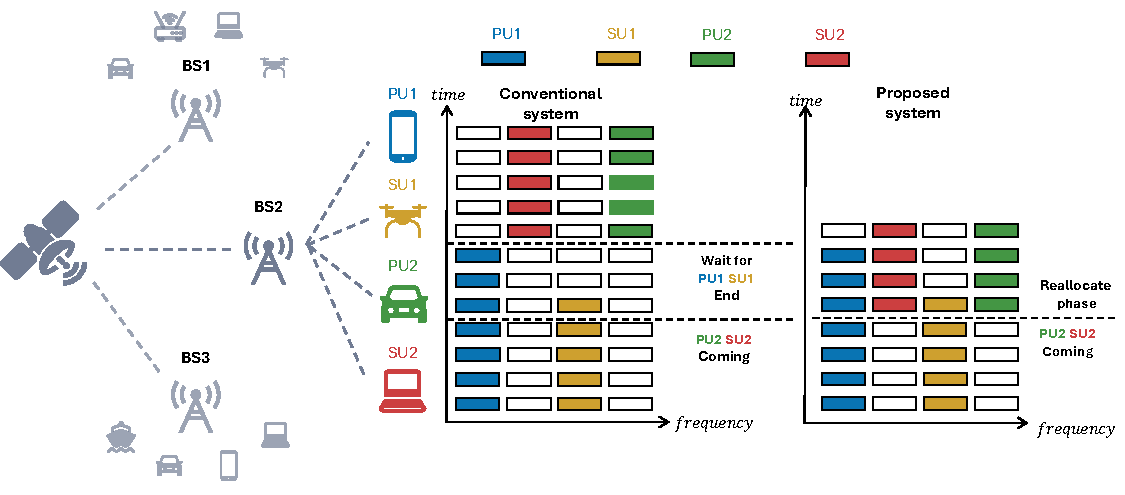
\includegraphics[width=6.5in]{Fig/Slide1.pdf}%
\caption{Comparison between the conventional spectrum allocation system and the proposed system utilizing a diffusion model for time domain signal prediction. On the left, various base stations (BS1, BS2, BS3) and devices (including primary users PU1, PU2, and secondary users SU1 and SU2) communicate with the help of satellite links. The middle section illustrates the conventional system, where spectrum allocation waits for ongoing communications (e.g., PU1, SU1) to end before reallocating spectrum, leading to inefficiencies. In contrast, the right section shows the proposed system, where the diffusion model predicts the end of current communications and the start of new ones (PU2, SU2), allowing for dynamic reallocation of spectrum resources. This proactive reallocation enhances spectrum utilization by reducing waiting times and optimizing the allocation phase.}
\label{fig_1}
\end{figure*}

\section{Simulation Setup and Data Generation}\label{sec:data}
A simulation setup is configured to simulate a dynamically changing indoor wireless environment, where multiple users attempt to share a fixed spectral channel resource through a single transmitter. For this experiment, we assume this resource to be 5 seconds of transmission with a bandwidth of 80 MHz centered at a carrier frequency of $f_c=5.25$~GHz. To enable realistic experiments, this work utilizes the packet and resource allocation framework provided by IEEE 802.11ax (High Efficiency/HE), also known as Wi-Fi 6 Wireless Local Area Network (WLAN), which features a multi-user version of orthogonal frequency-division multiplexing (OFDM) known as OFDMA. In OFDMA, the overall channel is divided into fixed time-frequency blocks called \textit{resource units} and allocated amongst the users \cite{data_ref10}. The data generation process is described below and summarized in Fig. \ref{fig_data1}.  

\subsection{Modeling User Entry and User Payload} 
To model realistic spectrum utilization, the arrival of new users into the virtual experiment is modeled as a Poisson queue, with a probability of user arrival expressed using a Poisson distribution as \cite{data_ref4}:
\begin{equation}
P(Arrivals=n) = \frac{e^{-\lambda t}\left(\lambda t\right)^n}{n!}
\end{equation}
where $t$ is the time in seconds (an integer), $\lambda$ is the average number of new users arriving per second, and $n$ is the possible number of users arriving at a given instant of time. For this experiment, the Poisson variable $\lambda$ is assumed to vary with time as $\lambda=\left\lfloor10+10\left|\sin{\left(\frac{\pi t}{T}\right)}\right|\right\rfloor$, where $T=5$~s is the simulation time. The variation of $\lambda$ as a function of time is plotted in Fig. \ref{fig_data2}. Each incoming user is randomly assigned one audio payload file drawn from a custom library of 113 music and speech recordings sourced from publicly available datasets \cite{data_ref1, data_ref2, data_ref5, data_ref6, data_ref7, data_ref8, data_ref9}. Audio payloads were chosen to reflect realistic data content diversity; binary representations of these files serve as the transmitted data bits. The original raw audio files are trimmed to a random length between $10^6$ and $8\times10^6$ samples. The edited audio file in “.wav” format and the corresponding binary data file are available for download at \cite{data_ref3}.
\begin{figure*}[!t]
\centering
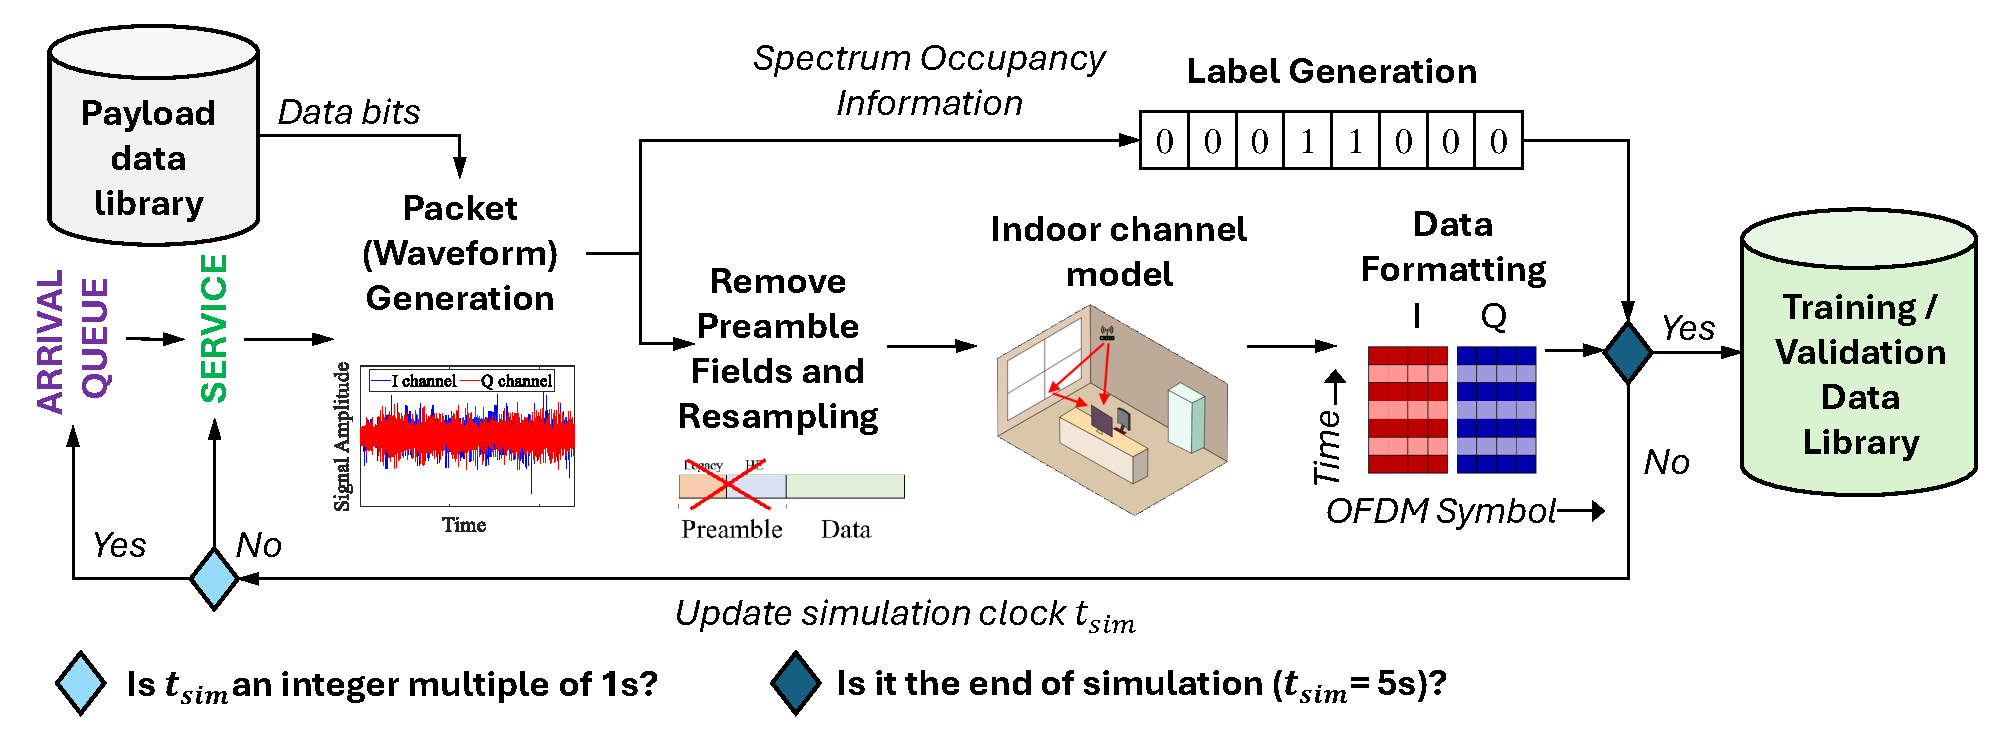
\includegraphics[width=6in]{Fig/Figure 6 - 240930.pdf}%
\caption{Overview of wireless signal data generation process.}
\label{fig_data1}
\end{figure*}

\begin{figure}
\centering
\subfloat[]{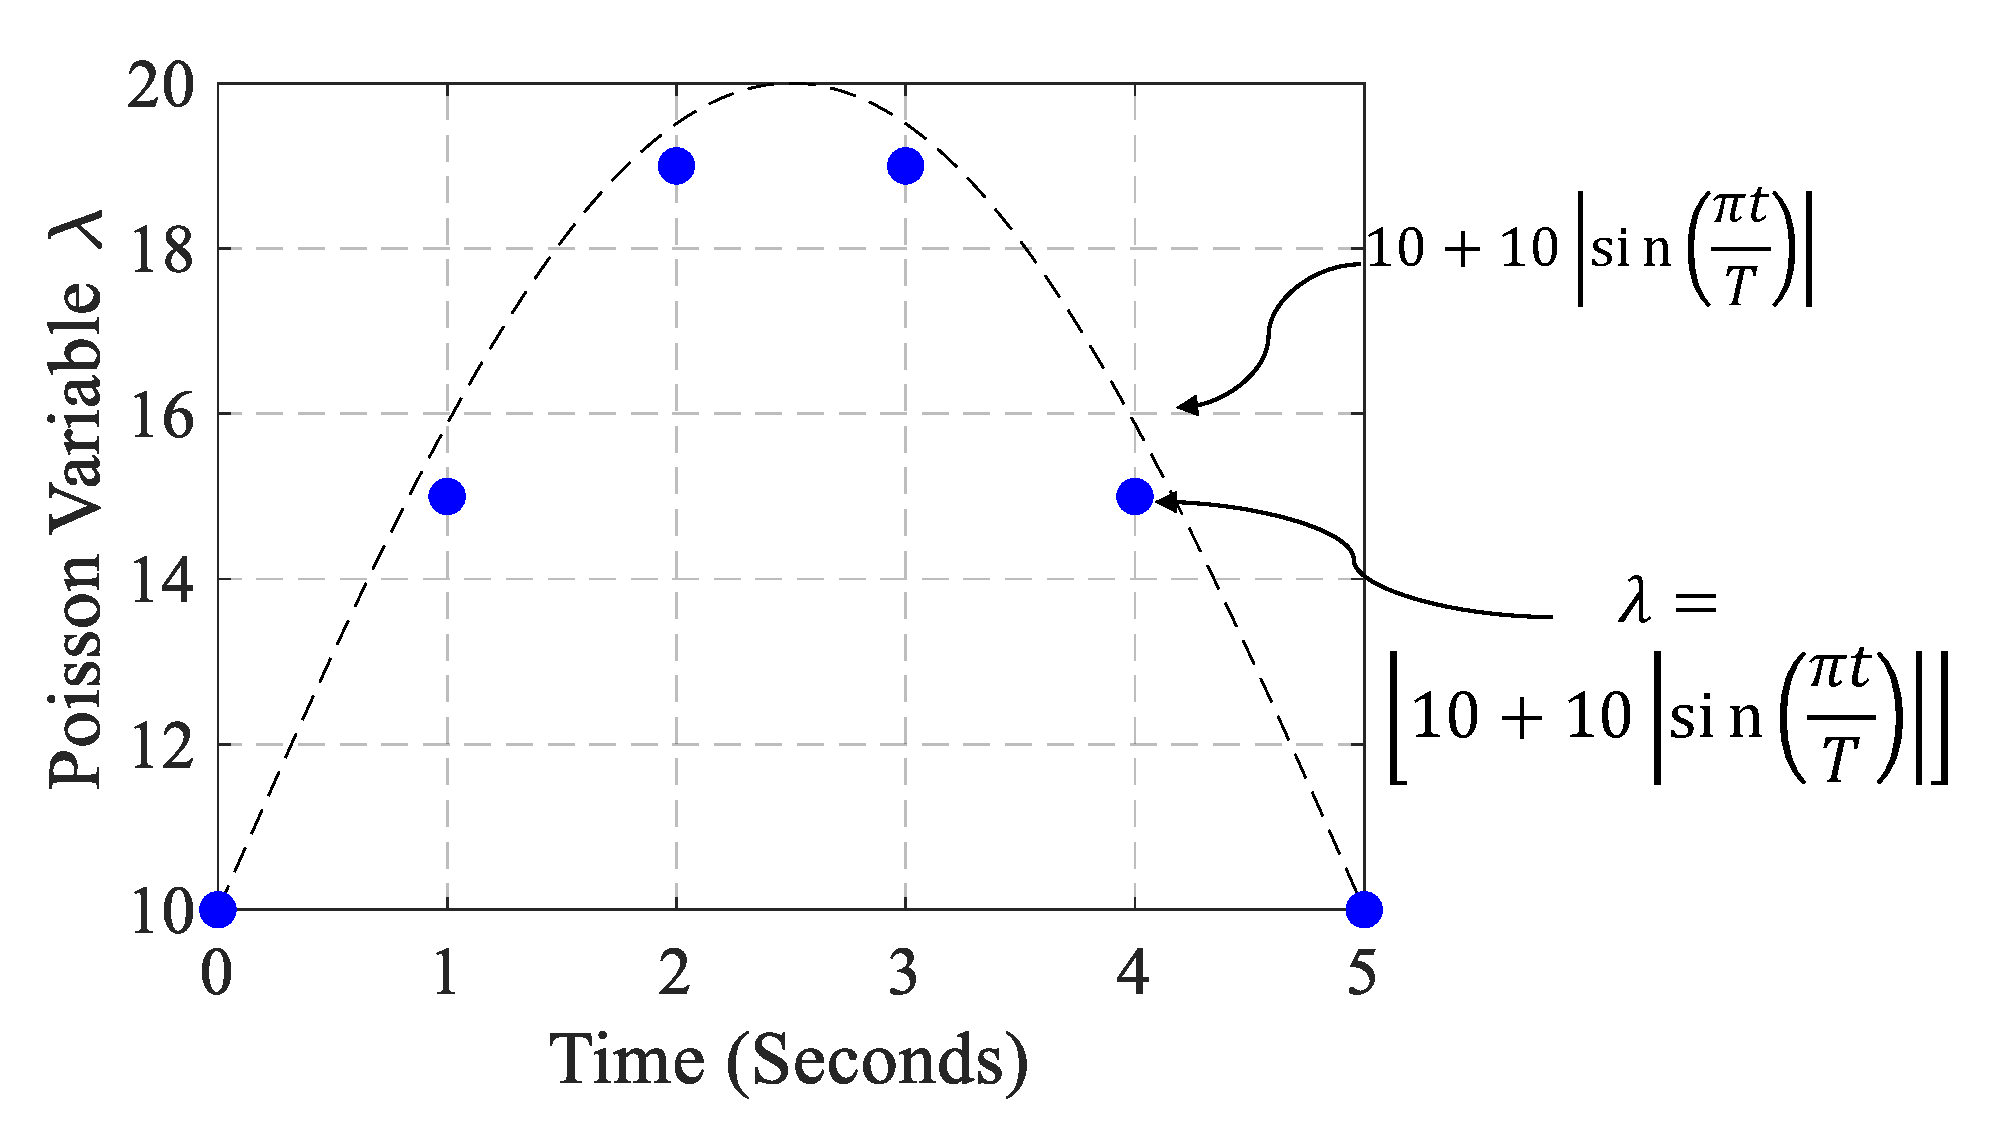
\includegraphics[width=3in]{Fig/Figure S1 - 240930.pdf}%
\label{fig_data2}}
\vfill
\subfloat[]{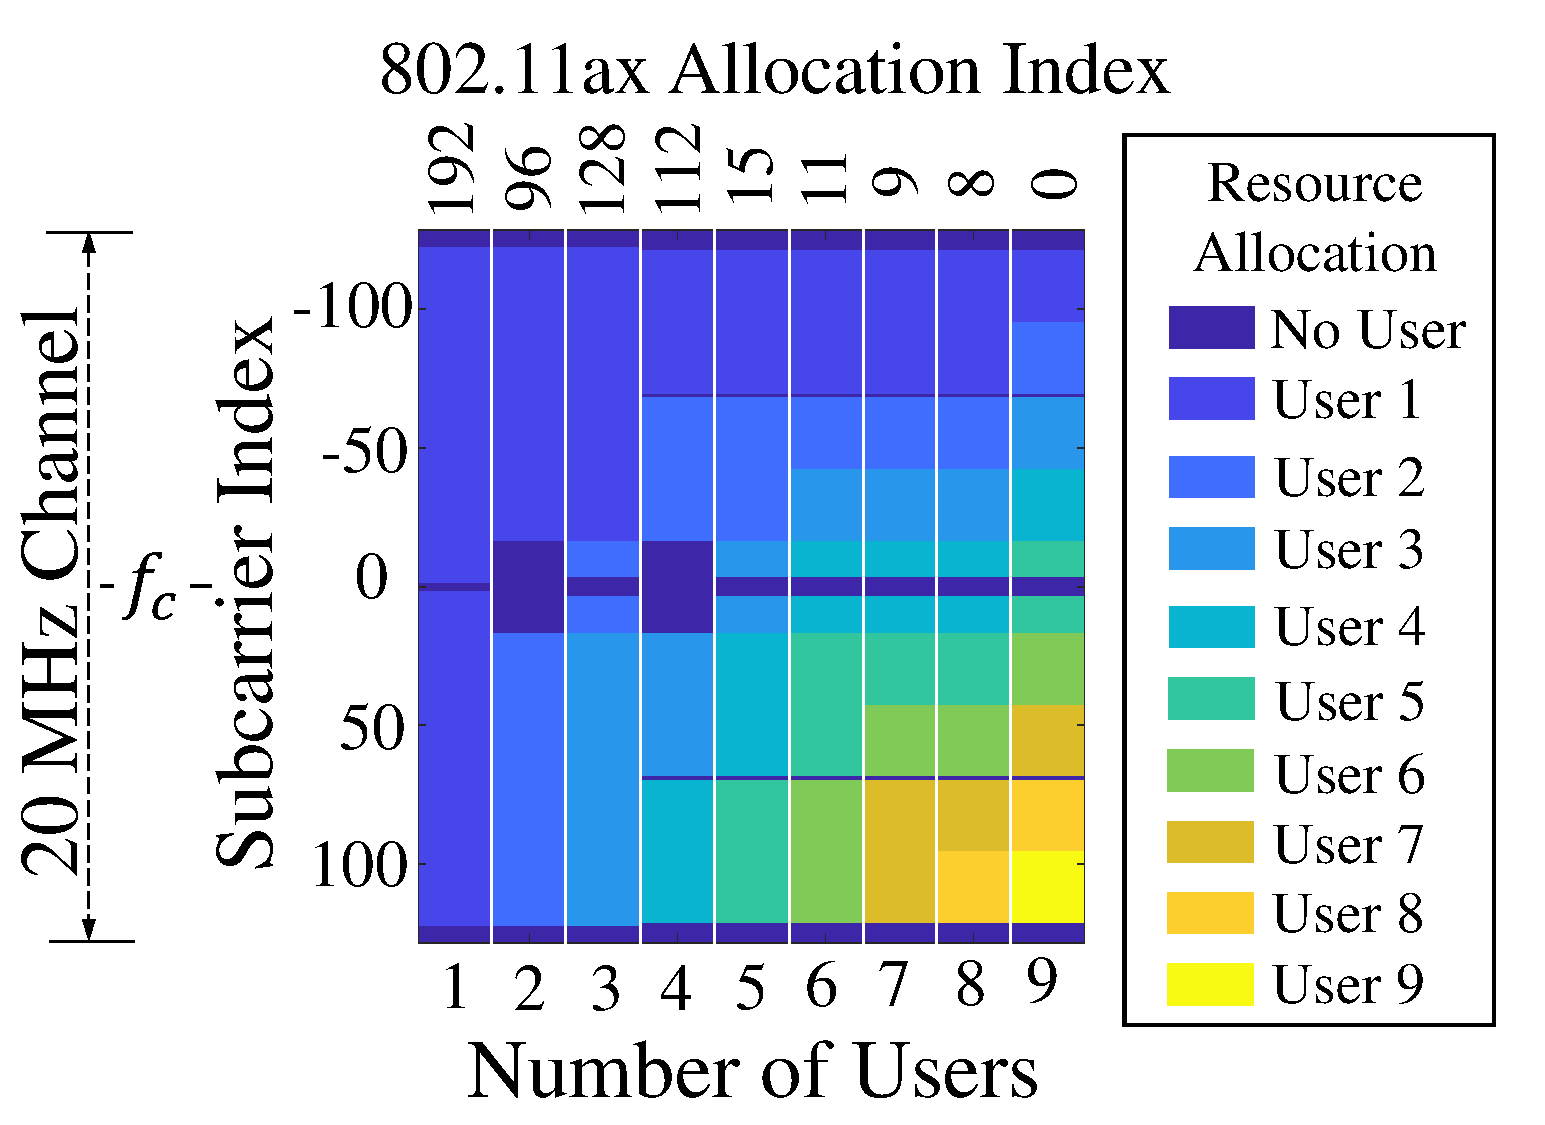
\includegraphics[width=3in]{Fig/Figure S2 - 240930.pdf}%
\label{fig_data3}}
\vfill
\subfloat[]{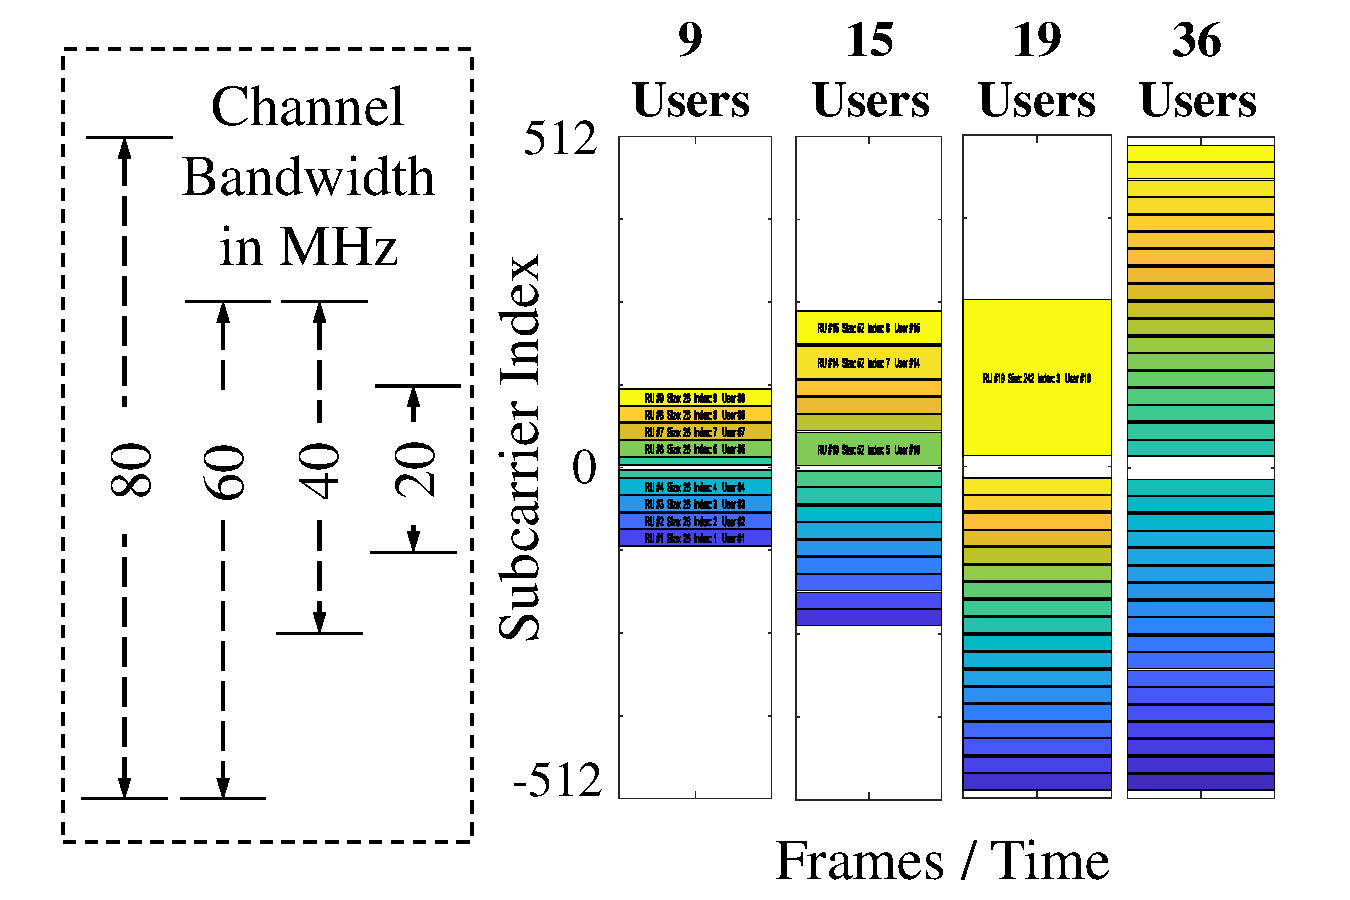
\includegraphics[width=3in]{Fig/Figure S3 - 240930.pdf}%
\label{fig_data4}}
\caption{(a) Values assigned to the Poisson Variable $\lambda$ as the data generation simulation progresses with time. (b) Allocation of OFDM sub-carriers and corresponding allocation index per 20 MHz sub-channel. In this work, each 20 MHz sub-channel supports a maximum of 9 users. (c) Allocation of OFDM sub-carriers and corresponding allocation index for the 80 MHz channel for 9, 15, 19, and 36 users, respectively. The subcarrier graph is generated using the MATLAB WLAN toolbox.}
\end{figure}

\subsection{Spectrum Allocation to Users}
The experiment is configured to support a maximum of 36 users attempting to utilize an 80 MHz channel. To meet the resource allocation process defined in the standard, a condition is imposed that the channel bandwidth is always occupied in multiples of 20 MHz sub-channels, with each supporting a maximum of 9 users. For instance, if the total number of users is below 9, only 20 MHz of the channel is utilized for transmission. The resource sharing strategy for each 20 MHz channel is predetermined in this work and constrained to 9 options, which in terms of \textit{allocation indices} defined in the 802.11ax standard would correspond to the set \{0, 8, 9, 11, 15, 96, 112, 128, 192\} (see Fig. \ref{fig_data3}) \cite{data_ref11}. If the number of users exceeds 9, the bandwidth is incremented by 20 MHz until that sub-channel is also occupied by 9 users. To illustrate, channel occupation over the maximum simulation bandwidth of 80 MHz is depicted for scenarios with 9, 15, 19, and 36 users, as shown in Fig. \ref{fig_data4}. 

\subsection{Simulation Setup}
As a user enters the experiment and is ready for transmission, they are also randomly allocated one of the modulation schemes listed in Table \ref{tab:data_table1}. The waveform packet is then generated using the MATLAB WLAN toolbox with an additional simulation constraint of APEP (Aggregate MAC Protocol Data Unit Pre-EOF Padding) length set randomly to 1000 or 1500 for each user. A continuous stream of packets is generated for 5~s with new users appearing every second; new users are allocated spectrum resources if available, transmit their payload, and exit the simulation upon completion. All transmitted waveforms are in the IQ baseband format and are sampled at a frequency of 80 MHz. To model realistic channel propagation, the IQ data is passed through an indoor channel model, and Additive White Gaussian noise (AWGN) is added, resulting in an SNR within the 20-25 dB range. For each five-second simulation, the channel is selected randomly from Wi-Fi standard compliant models, named Models A-F, available in MATLAB’s WLAN toolbox \cite{data_ref12}. Some simulation settings involving channel conditions include 0-2 walls with pathloss effects captured and 1-2 walls with pathloss and shadowing captured. A random transmitter-receiver distance between 2-5~m is used, and the SNR is restricted to between 20 and 25 dB. The channel coding is set to LDPC for all cases, and the number of space-time streams is set to 1. These parameter combinations yielded 30 distinct simulated channel environments — realizations of the standard channel models under a common single-transmitter traffic model — spanning a representative range of indoor propagation conditions. While this set does not exhaustively cover all real-world environments, it provides a controlled basis for validating the proposed framework. A flowchart of the simulation process is provided in Fig. \ref{fig_data1}.  

\subsection{Dataset Formatting and Labeling}

An ideal receiver captures the transmitted data after propagation through the channels. The receiver removes packet headers, and the time-domain payload waveform is arranged such that each OFDM symbol in the waveform corresponds to one row in a matrix. Each data element’s real and imaginary components, i.e., I and Q components, are further separated into different matrices. As an example, and for a sense of scale, one 5-second simulation resulted in a data matrix of size $303459 \times 1024$. Labels are generated for each row in the data matrix, corresponding to the spectrum occupancy information. Each label consists of eight fields representing one 10 MHz subchannel within the 80 MHz band of interest. A value of 0 or 1 within a field indicates that the corresponding 10 MHz sub-channel is unoccupied or occupied, respectively. 
Sixty data files are generated—30 for training and 30 for validation—across each indoor channel model.


\begin{table}[!t]
\caption{Available Modulation and Coding Schemes for Transmission
\label{tab:data_table1}}
\centering
\begin{tabular}{|c|c|}
\hline
MCS Value & Modulation and Coding\\
\hline
2 & QPSK with 1/2 coding rate\\
3 & 16-QAM with 1/2 coding rate\\
4 & 16-QAM with 3/4 coding rate\\
5 & 64-QAM with 2/3 coding rate\\
6 & 64-QAM with 3/4 coding rate\\
7 & 64-QAM with 5/6 coding rate\\
8 & 256-QAM with 3/4 coding rate\\
\hline
\end{tabular}
\end{table}

\section{Model and Methods}\label{sec:methods}

\begin{figure}[!t]
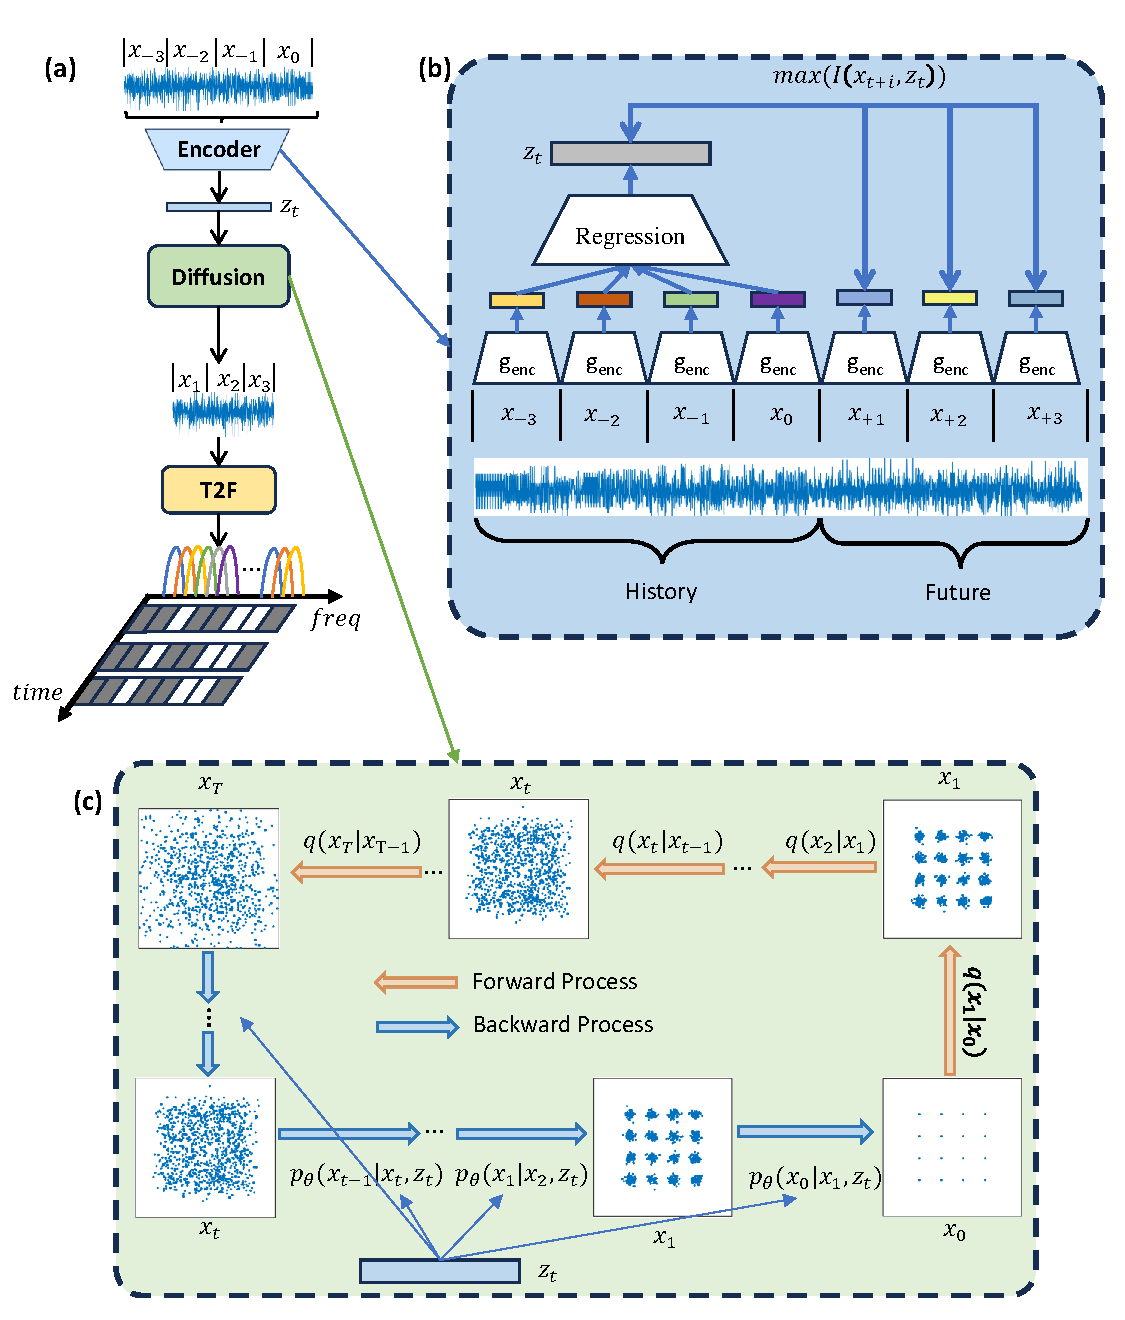
\includegraphics[width=3.3in]{Fig/Slide2.pdf}
\caption{System Diagram (schematic; four history frames are drawn for illustration, while the deployed configuration uses a 128-frame history). (a) System Flow. The input is the historical signal $\left[x_{-3},..,x_0\right]$, compressed by the Encoder (Latent Space Extractor) as $z_t$. This latent vector provides the condition of the diffusion model. The diffusion model generates the future signal. The T2F model predicts the future frequency occupation by taking the generated future time domain signal. (b) Encoder (LSE) training process from \cite{model_ref1}. (c) The latent vector $z_t$ conditions the diffusion process for future projections.}
\label{fig_model_1}
\end{figure}

The framework operates directly on raw time-domain signals, whose preserved modulation structure allows the downstream classifier to infer sub-channel occupancy at the resolution of individual OFDM frames (approximately 13 $\mu$s). Fig. \ref{fig_model_1}a illustrates our model's overall flow, specifically designed to meet the high bandwidth demands of contemporary wireless communication. As frequency bands widen, the sheer volume of sample points becomes overwhelming, making directly integrating raw signal waveforms into our prediction framework impractical.

The critical component in reducing the data volume and enabling the model to operate across multiple environments is the Latent Space Extractor (LSE), whose training process is depicted in Fig. \ref{fig_model_1}b. Detailed in the "Method" section, the LSE is a time-series processing model specifically designed to address the complexities of spectrum prediction. Its ability to condense complex, high-dimensional data into a streamlined, lower-dimensional latent space \cite{model_ref1} is essential for reducing the computational load in the subsequent diffusion model.

The encoder within the LSE effectively distills the context of historical raw data, lowering computational demands. This enhances the model's ability to capture temporal patterns in user transmission behavior while keeping computational resources in check — an advancement not possible with previous methods relying on matched filters or signal power analysis.

We utilize the diffusion model to generate future time-domain signals because it enables precise predictions for each time frame. Unlike traditional methods that rely on power information or matched filter detection and can only make predictions over long time ranges \cite{intro_ref7, intro_ref8, intro_ref9}, time-domain signal prediction provides granular, frame-by-frame forecasts. By conditioning the diffusion model on a history encoder, the framework can anticipate user departure and arrival events at the OFDM frame level, reflecting the model's capacity to capture temporal patterns in user transmission behavior, thereby enhancing real-time spectrum management.

Fig. \ref{fig_model_1}c illustrates the forward and backward processes within the diffusion model used for spectrum prediction. The forward process, depicted by orange arrows, represents the gradual addition of noise to the signal, transitioning from the clean signal $x_0$ to the noisy samples $x_T$. The backward process, shown by blue arrows, illustrates how the model denoises the signal step-by-step, starting from $x_T$ and working back to $x_0$. The guidance $z_t$ is fed into the backward process to improve prediction accuracy, refining the signal at each step. This iterative refinement allows the model to reconstruct a clear signal from a noisy input, which is crucial for accurate spectrum utilization predictions. 

\subsection{Encoder Model}
The Contrastive Predictive Coding (CPC) method excels at extracting meaningful features from unlabeled data, making it highly effective for transfer learning across various downstream tasks. This self-supervised learning approach capitalizes on abundant unlabeled data and enhances adaptive system design, interference mitigation, and spectrum sensing in wireless communication networks. CPC's ability to distinguish between signal and noise and its potential to improve signal quality positions it as a powerful tool for advancing wireless signal processing. This capability enables the development of more efficient and reliable wireless communication systems.

The CPC model comprises two primary elements: an encoder and an autoregressive context prediction model. The encoder, denoted as $f_{enc}$, transforms each input context window $x_t$ into a latent representation within a fixed-dimensional embedding space $z_t=f_{enc}\left(x_t\right)$. These latent embeddings capture the essential features of the input data, facilitating the subsequent prediction tasks. Subsequently, an autoregressive model $g_{ar}$ compresses the $N$ history latent representations into a lower dimensional latent feature vector, $c_t$, given by:
\begin{equation*}
    c_t=g_{ar}\left(z_t,z_{t-1},z_{t-2},\cdots,z_{t-N+1}\right)
\end{equation*}

The objective is to model a density ratio that effectively preserves the mutual information between a designated future context window and the corresponding latent vector, which is represented by:
\begin{equation}
\begin{aligned}
    M_{\theta_k}\left(x_{t+k},\ c_t\right) = &e^{\left(z_{t+k}^T \times W_{\theta_k} c_t\right)}\\
    &\propto I\left(x_{t+k},c_t\right)\propto\frac{p\left(x_{t+k}\middle| c_t\right)}{p\left(x_{t+k}\right)}
\end{aligned}
\end{equation}


In this framework, $W_{\theta_k}$ represents the trainable model that projects the latent feature vector $c_t$ into a prediction vector. This projection is designed to maximize mutual information $I\left(x_{t+k},c_t\right)$ with the $k^{th}$ future context window, $z_{t+k}$, which is the encoded vector of $x_{t+k}$: 

\begin{equation}
    z_{t+k}^T=f_{enc}\left(x_{t+k}\right)
\end{equation}

$I\left(\cdot\right)$ is the mutual information entropy function quantifying the data probability distribution $\frac{p\left(x_{t+k}\middle| c_t\right)}{p\left(x_{t+k}\right)}$.

The encoder and the autoregressive model are jointly trained based on the infoNCE loss \cite{model_ref1} defined as:
\begin{equation*}
    \mathcal{L}_N = -\mathbb{E}_N\left[\log\frac{M_{\theta_k}(x_{t+k}, c_t)}{\sum_{x_i\in X}M_{\theta_k}(x_i, c_t)}\right]
\end{equation*}

where $X=\{x_1,x_2,\cdots,x_N\}$ is a set of samples that contains one positive sample $p\left(x_{t+k}\middle| c_t\right)$ and $N-1$ negative samples from $p\left(x_{t+k}\right)$. This loss classifies the positive sample. The optimal value for $M_{\theta_k}\left(x_{t+k},c_t\right)$ is proportional to $\frac{p\left(x_{t+k}\middle| c_t\right)}{p\left(x_{t+k}\right)}$ and depends on the choice of the number of negative samples. For more details, see the Supplemental Material, which includes training and testing procedures.

The encoder's convolutional backbone employs non-causal (centered) convolution kernels. This choice is motivated by the structure of Orthogonal Frequency Division Multiplexing (OFDM) symbols: each symbol is generated by an IFFT with a cyclic prefix, so the informative structure within a received frame is symmetric and cyclic rather than strictly left-to-right sequential. A centered kernel treats samples on both sides of a position symmetrically and therefore matches this within-symbol structure, whereas a causal kernel would impose an artificial temporal ordering inside each frame that the cyclic symbol structure does not possess. We emphasize that non-causality here refers only to kernel centering within already-received history frames: at inference, the encoder input consists exclusively of past samples, and no future samples are available to or used by the encoder.

\subsection{Diffusion Model}
The purpose of the diffusion model in this work is to generate appropriate future temporal domain wireless communication waveforms based on the available prior information. Historical data is incorporated in the set $X=\{\ x_t\in\mathbb{R}^d\ |t=-T_{hst},-T_{hst}+1,\cdots,0\}\in\mathbb{R}^{\left(T_{hst}+1\right)\times d}$, where $d$ is the number of sampling points of the incoming wireless signal in each context window, $T_{hst}$ is the length of the observed historic context window size while the current timestamp is $t=0$. Similarly, prediction data is incorporated in the set $Y=\{\ y_t\in\mathbb{R}^d|t=1,2,\cdots,T_{pred}\}\in\mathbb{R}^{T_{pred}\times d}$, where $T_{pred}$ is the maximum number of the predicted frames.

During the diffusion process, the future signals $y_t^{\left(0\right)}$ are gradually reduced to a noise distribution given by the set $\left(y_t^{\left(0\right)},y_t^{\left(1\right)},y_t^{\left(2\right)},\cdots,y_t^{\left(N\right)}\right)$, where $N$ is the maximum number of diffusion steps, $y_t^{\left(0\right)}$ is a sample from the latent distribution $q\left(y_t^{\left(0\right)}\middle| X\right)$, and $X$ is history information.

The role of the diffusion model is to generate appropriate future time-domain signal waveforms, conditioned by the latent feature $f$, which is a vector extracted by the encoder from the history $X\in \mathbb{R}^{\left(T_{hst}+1\right)\times d}$. The generation process is the reverse flow of the diffusion process where new initial points are sampled from the noise distribution $p\left(y_t^{\left(N\right)}\right) \sim \mathcal{N}\left(0,I\right)$ that approximates $q\left(y_t^{\left(N\right)}\right)$, which is the last step of the forward process. The input traverses the reverse Markov process to generate the corresponding waveform. The reverse flow is modeled by a neural network parameterized by $\theta$. 

The reverse Markov process can be formulated as:
\begin{equation}
    \begin{aligned}
        p_\theta\left(y_t^{\left(0:N\right)}\middle| f\right)&=p\left(y_t^{\left(N\right)}\right)\prod_{n=1}^{N}{p_\theta\left(y_t^{\left(n-1\right)}\middle| y_t^{\left(n\right)},f\right)} \\
        &=p\left(y_t^{\left(N\right)}\right)\prod_{n=1}^{N}\mathcal{N}\left(y_t^{\left(n\right)};\mu_\theta\left(y_t^{\left(n\right)},n,f\right),\beta_nI\right)
    \end{aligned}
\end{equation}

where $\mu_\theta$ represents the mean of the random distribution, $f$ is the latent feature of the history information, $p\left(y_t^{\left(N\right)}\right)$ is a standard normal distribution $\mathcal{N}\left(0,I\right)$ representing the initial distribution of $y_t^{\left(N\right)}$, and $\beta_n,\, n=1,2,\cdots,N$ is a hyper-parameter that controls the diffusion rate of the process. For clarity, the rest of the paper will use the entire sequence $T_{pred}$ of future time frames $Y^{\left(n\right)}$, where $n$ indicates the $n^{th}$ forward/reverse step, instead of one single time frame $y_t^{\left(N\right)}$.

The reverse diffusion process is trained by minimizing a simplified loss function at each reverse step $n\in\left\{1,\ 2,\ \cdots,\ N\right\}$:
\begin{equation}
    L\left(\theta\right)=\mathbb{E}_{n,\ Y^{\left(0\right)},\epsilon}\left[ \| \epsilon - \epsilon_{\theta}(Y^{\left(n\right)},n,\ f) \|^2 \right]
\end{equation}
which is derived by maximizing the log-likelihood of the final probability distribution $E\left[\log{\left(p_\theta\left(Y^{\left(0\right)}\right)\right)}\right]$. This log-likelihood is bounded below by the variational lower bound:
\begin{equation}
\begin{aligned}
    &\mathbb{E}\left[\log{p_\theta\left(Y^{\left(0\right)}\right)}\right]\geq \\ &\mathbb{E}_q\left[\log p\left(Y^{\left(N\right)}\right)+\sum_{n=1}^{N}\log{\frac{p_\theta\left(Y^{\left(n-1\right)}\middle| Y^{\left(n\right)},\ f\right)}{q\left(Y^{\left(n\right)}\middle| Y^{\left(n-1\right)}\right)}}\right]
\end{aligned}
\end{equation}

Based on this simplified loss function, the training and sampling algorithm can be summarized as follows:
\begin{algorithm}[H]
\caption{Training}\label{alg:alg1}
\begin{algorithmic}
\STATE 
\STATE {\textbf{Repeat}}
\STATE \hspace{0.5cm}Sample $ Y^{\left(0\right)}\sim q_{data}\left(Y^{\left(0\right)}\right) $
\STATE \hspace{0.5cm}Sample $ f\sim g_{enc}\left(X^{\left(0\right)}\right) $
\STATE \hspace{0.5cm}Sample $ n\sim Uniform\left(\left\{1,\ \ 2,\ \cdots,\ \ N\right\}\right) $
\STATE \hspace{0.5cm}Sample $ \epsilon\sim\mathcal{N}\left(0,I\right) $
\STATE \hspace{0.5cm}Compute $ \nabla [ \sum_{y_i^{\left(0\right)}\in Y^{\left(0\right)}} \| \epsilon- $
\STATE \hspace{3cm}$\epsilon_\theta\left(\sqrt{\bar{\alpha_n}}y_i^{\left(0\right)}+\sqrt{1-\bar{\alpha_n}}\epsilon,\, n,\, f\right) \|^2 ] $
\STATE \hspace{0.5cm} Gradient Descent
\STATE \textbf{Until} converged
\end{algorithmic}
\label{alg1}
\end{algorithm}

\begin{algorithm}[H]
\caption{Sampling}\label{alg:alg2}
\begin{algorithmic}
\STATE Sample $ f\sim g_{enc}\left(X^{\left(0\right)}\right) $
\STATE $Y^{\left(N\right)}\gets\{{y}_i^{\left(N\right)}\}\sim\mathcal{N}\left(0,I\right)$
\STATE \textbf{for} $n=N\cdots 1 $ \textbf{do}
\STATE \hspace{0.5cm}Sample $ Y^{\left(n-1\right)}\sim p_\theta\left(Y^{\left(n-1\right)}\middle| Y^{\left(n\right)},f\right)  $
\STATE \textbf{end for}
\STATE \textbf{return}  $ Y^{\left(0\right)} $
\end{algorithmic}
\label{alg2}
\end{algorithm}

\subsection{System Fine-Tuning}
After each sub-model has been trained separately, the whole system is considered for fine-tuning to reduce the sensitivity of the T2F-CNN model to errors. These errors mainly arise from the distance between the diffusion model’s sampling and ground-truth positions in the signal’s intrinsic probability distribution. The diffusion model’s parameters are frozen, while the parameters of the encoder and the T2F model are set to be trainable. The history signal is fed into the encoder, generating the latent space vector as the condition of the diffusion model, which samples a new $Y_t^{\left(N\right)}$ from the normal distribution and gradually denoises it to $Y_t^{\left(0\right)}$. The $Y_t^{\left(0\right)}$ is then sent to the T2F-CNN model to predict the future spectrum. The Cross-Entropy Loss between $\hat{S}\left(t,\ f\right)$ and $S\left(t,\ f\right)$ is used as the loss for fine-tuning, where $\hat{S}\left(t,\ f\right)$ is the predicted spectrum occupation for future time frames and $S\left(t,\ f\right)$ is the actual spectrum occupation for future time frames. To reduce sensitivity to errors introduced by the diffusion model, a weighted cross-entropy loss is used during fine-tuning. Correctly predicted positions are down-weighted by a factor of 0.1 to focus the gradient signal on incorrectly predicted sub-channel states. This formulation can be expressed as:
\begin{equation}
    \begin{aligned}
        \mathcal{L}=&0.1\times\mathbbm{1}\left(\hat{S}=S\right)\times\mathcal{L}_{CrossEntropy}\left(p\left(\hat{S}\right),\ p\left(S\right)\right) \\
        & +1\times\mathbbm{1}\left(\hat{S}\neq S\right)\times\mathcal{L}_{CrossEntropy}\left(p\left(\hat{S}\right),\ p\left(S\right)\right)
    \end{aligned}
\end{equation}
where the $\mathbbm{1}$ is the indicator function. Here $\hat{S}$ denotes the hard occupancy decision obtained by thresholding the T2F output probability at 0.5; the indicator masks are non-differentiable and act as fixed per-element weights, so the gradient propagates through the cross-entropy terms only, with weight 0.1 on correctly predicted positions and weight 1 on incorrectly predicted ones. This asymmetric weighting encourages the encoder and T2F model to correct diffusion-induced errors without disrupting already-correct predictions.

Table~\ref{tab:model_params} summarizes the parameter counts 
for each module in the proposed framework.

\begin{table}[h]
\centering
\caption{Model Parameter Summary}
\label{tab:model_params}
\begin{tabular}{lcc}
\hline
\textbf{Module} & \textbf{Parameters} & \textbf{Description} \\
\hline
Encoder        & 0.1B & 1D Conv + Transformer \\
Diffusion Model & 0.1B & Transformer with conditioning\\
T2F CNN        & 17M & 1D Conv \\
\hline
\textbf{Total} & \textbf{0.2B} & — \\
\hline
\end{tabular}
\end{table}

\section{Results}
\subsection{Encoder (LSE) Model Evaluation}
In this work, we employ a contrastive learning method that enables our prediction system to operate effectively across a wide range of wireless communication environments. Unlike previous state-of-the-art spectrum prediction models focusing on specific frequency bands or static environments, our encoder adaptively compresses and extracts features from diverse and dynamic signal environments. This flexibility suggests that the model may generalize to new wireless environments with limited or no retraining, a property that we examine directly through the zero-shot transfer experiment reported in Section~\ref{sec:zeroshot}; few-shot adaptation remains a direction for future work \cite{result_ref1, result_ref2, result_ref3}.

Our investigation into the Latent Space Extractor (LSE) leverages a contrastive learning technique inspired by Contrastive Predictive Coding (CPC) \cite{model_ref1}, a method renowned for its ability to create efficient data representations. We explore the LSE's performance across various parameter settings, particularly how different historical signal intervals and latent space dimensions impact the model's precision and efficiency.

\begin{figure*}[!t]
\centering
\subfloat[]{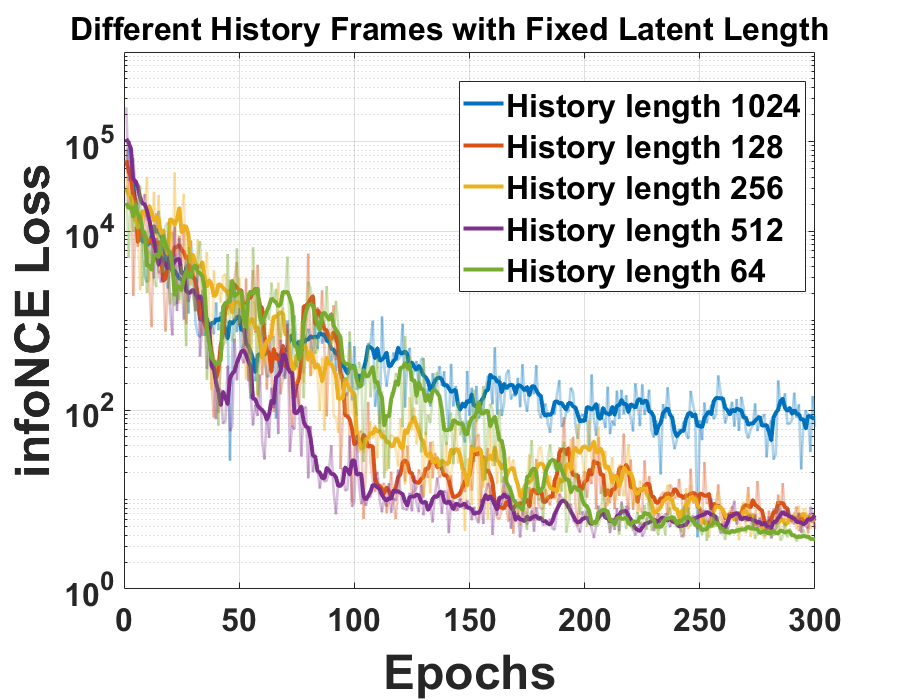
\includegraphics[width=2.2in]{Fig/contrast_test_hist_len.png}%
\label{fig_res1}}
\hfil
\subfloat[]{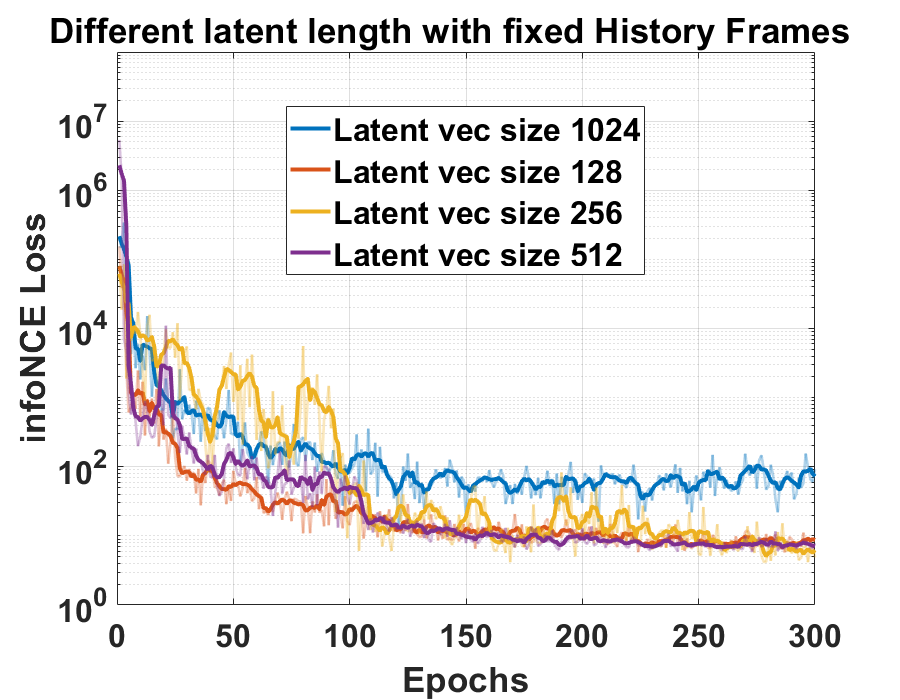
\includegraphics[width=2.2in]{Fig/contrast_test_feature_len.png}%
\label{fig_res2}}
\hfil
\subfloat[]{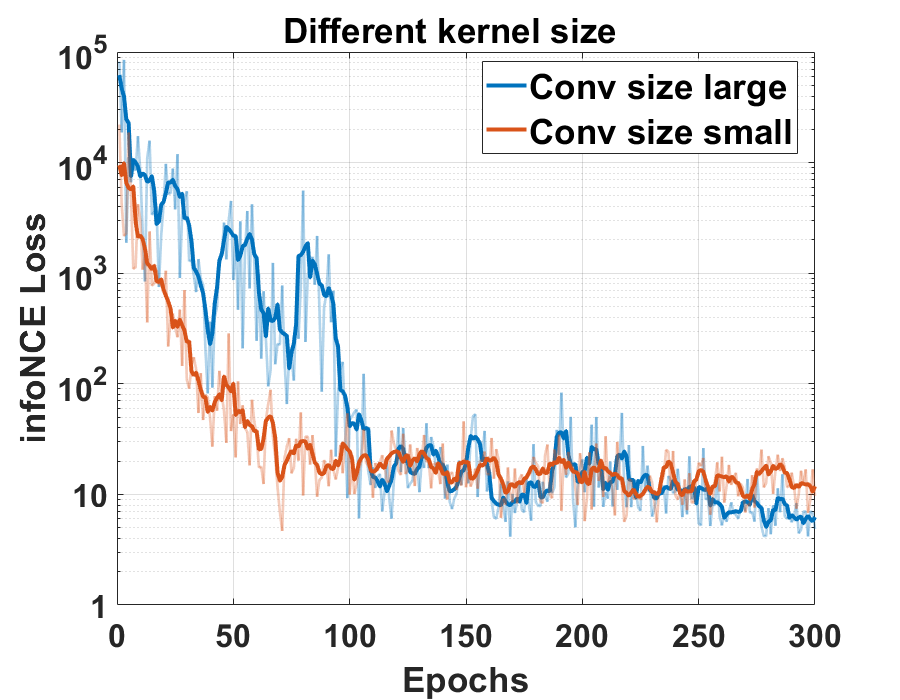
\includegraphics[width=2.2in]{Fig/contrast_test_conv_size.png}%
\label{fig_res3}}
\vfill
\centering
\subfloat[]{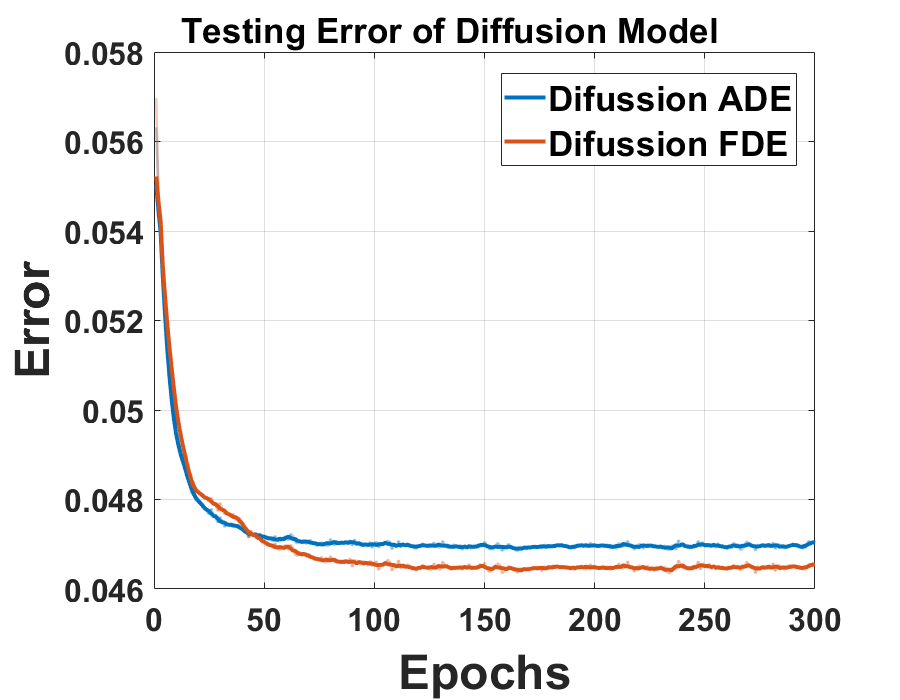
\includegraphics[width=2.2in]{Fig/Testing errors.png}%
\label{fig_res4}}
\hfill
\subfloat[]{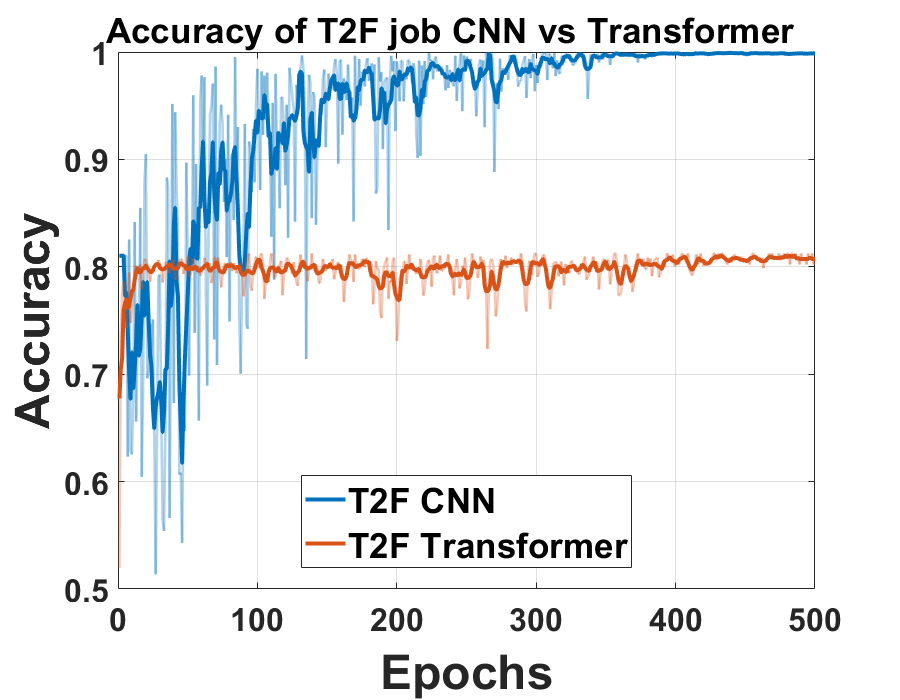
\includegraphics[width=2.2in]{Fig/testing.png}%
\label{fig_res5}}
\hfill
\subfloat[]{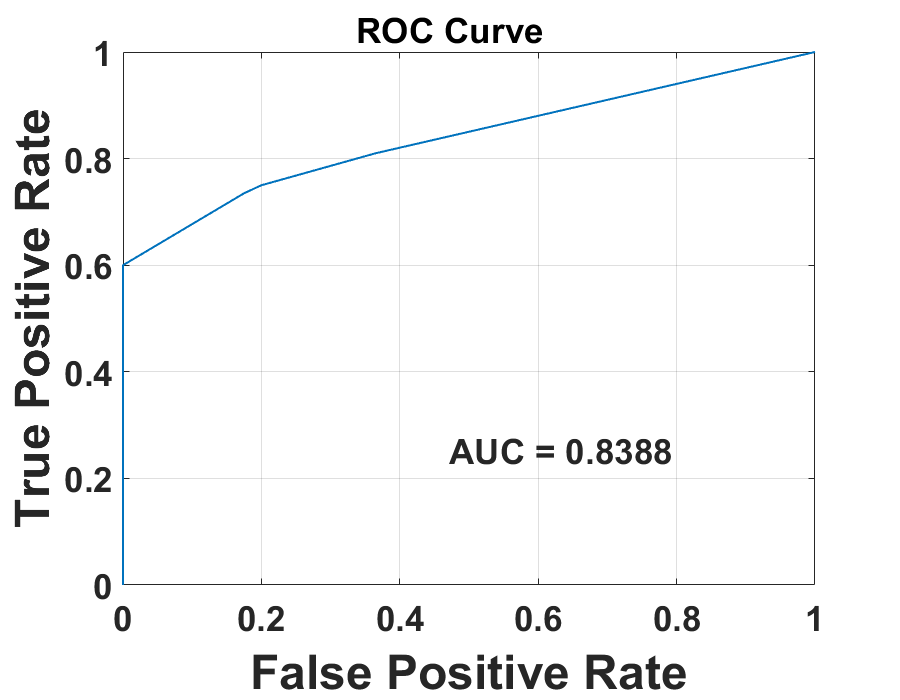
\includegraphics[width=2.2in]{Fig/untitled.png}%
\label{fig_res6}}

\caption{Validation Results. (a) Encoder testing results with different history time frame lengths. (b) Encoder testing results with different latent space vector lengths. (c) Encoder testing results with large ([513, 385, 257, 129, 65]) versus small ([7, 7, 9, 9, 11]) convolution kernel sizes. (d) Latent Diffusion Model Validation Average Displacement Error (ADE) and Final Displacement Error (FDE). (e) T2F model validation comparison between CNN-based model and transformer-based model. (f) ROC curve of the system-level final frequency-block predictions, obtained by sweeping the prediction confidence threshold}
\label{fig_result}
\end{figure*}

Fig.~\ref{fig_res1} illustrates the validation performance of the Contrastive Predictive Coding (CPC) model, highlighting the effects of varying the number of historical signal frames while maintaining a constant latent space vector length of 128. The feature extractor, trained across diverse wireless environments, significantly enhances the model's resilience in spectrum-sharing scenarios. Negative samples are carefully selected from a heterogeneous signal waveform pool, deliberately excluding those closely related to the positive sample's immediate environment.

Adapting the CPC model to handle 1024 historical OFDM frames necessitates reducing the learning rate and applying a stricter gradient clipping threshold, resulting in a longer and more complex training process. However, the marginal performance improvements do not sufficiently justify the added complexity and extended training time associated with the increased number of historical frames. This finding underscores the need to balance model complexity and performance gains, especially with extensive temporal datasets typical of wireless communication signals. Similar conclusions are drawn regarding the impact of different latent feature vector lengths ($z_t$ in Fig. \ref{fig_model_1}b), as shown in Fig. \ref{fig_res2}.

Our second analysis compares the effects of varying convolution kernel sizes within the encoder, as shown in Fig. \ref{fig_res3}. The kernel sizes examined, [513, 385, 257, 129, 65] versus [7, 7, 9, 9, 11], along with a consistent stride pattern [3, 3, 3, 3, 3] and dilation configuration [5, 5, 5, 3, 3], indicate that kernel size does not significantly affect the model's convergence ability. This result may be attributed to the sizeable receptive field provided by the cumulative effect of multiple convolutional layers. Specifically, the receptive field for the final layer in our Conv1D Autoencoder model spans 959 elements. This expansive receptive field ensures that the output at this layer is influenced by a broad segment of the input sequence, encompassing 959 elements, comparable to the 1024 points per time frame in the original Orthogonal Frequency Division Multiplexing (OFDM) signal modulation. Such a broad receptive capacity highlights the model's proficiency in capturing long-range dependencies and intricate patterns throughout the data, a capability essential for tasks that require temporal patterns of complex contextual information.

\subsection{Diffusion Model Evaluation}
In this analysis, we elucidate our diffusion model's efficacy, specifically designed to forecast spectrum utilization. By incorporating an advanced diffusion process, the model gradually learns the intrinsic distribution of signals, even as they are modulated in complex ways and distorted by wireless channels. The sampled futures therefore reflect both the stochastic user dynamics and the channel-induced distortions implied by the conditioning history.

Unlike straightforward methods that predict future spectrum utilization, our diffusion model generates potential future time-domain signals aligned with the ground truth within the signal's probability distribution. The predicted waveforms are the basis for determining spectrum occupation, categorized as vacant (label 0) or in use (label 1). The model fine-tunes these generated values through a progressive denoising sequence, enabling the predicted waveform to closely approximate the actual future waveform. Based on the input historical signal data, this gradual denoising process allows the diffusion model to effectively predict when currently transmitted information will end and when new users and information will begin transmission.

The latent diffusion model is trained using a control factor, specifically the latent space vector $z_t$, obtained from the pre-trained encoder discussed earlier. The generated future signal is then passed to the T2F (Temporal-to-Frequency) model, described later in this section to predict future spectrum utilization. The MSE loss on the normalized dataset converges to approximately 0.6, which is consistent with the stochastic nature of the diffusion model's output: because the model generates samples from a distribution rather than producing a deterministic signal, residual variance relative to any single ground-truth waveform is expected. Empirically, this decomposition holds on the validation environments: a single sampled future incurs a mean squared error of 0.57 (median across environments), while the ensemble mean over the 20 samples attains 0.35 — matching the intrinsic variance of the signal itself (0.34), the irreducible floor arising from random payload content and channel noise. The gap between the single-sample and ensemble figures thus measures the diversity of the sampled futures rather than a systematic reconstruction error, and the meaningful evaluation of predictive skill is therefore conducted downstream, at the occupancy level, via AUC and F1. To monitor the performance of the diffusion model, we use the Average Displacement Error (ADE) and Final Displacement Error (FDE), as shown in Fig. \ref{fig_res4}. ADE calculates the average error between all the ground truth signals and the predicted signals in future communications. At the same time, FDE measures the displacement between the end time frame of the ground truth and the predicted signal's last time frame. The results show that both ADE and FDE converge to 0.047. Typically, FDE exceeds ADE because prediction errors accumulate over longer horizons. The convergence of ADE and FDE to 0.047 in our experiments suggests that the model's per-frame error does not increase substantially across the 32-frame prediction window, indicating stable temporal extrapolation. This horizon was limited by available GPU memory, not by model degradation, and longer-horizon evaluation is a natural direction for future work.

\subsection{Temporal to Frequency Model Evaluation}
The Temporal-to-Frequency Model (T2F Model) undergoes a pre-training process using a dataset of raw wireless signals and is designed to process the 32 OFDM time frames generated by the diffusion model. Instead of labeling each sub-carrier of the signal, the T2F model classifies the frequency domain into eight sub-blocks, each comprising multiple sub-carriers. This approach streamlines the classification process by focusing on sub-blocks rather than individual sub-carriers, thus enhancing efficiency without sacrificing critical frequency domain information. This method aligns with the practical usage in Wi-Fi and LTE protocols, where multiple sub-carriers are typically allocated to a single user.

Partitioning the frequency bands into sub-blocks is applicable across various wireless communication scenarios, where each sub-block can serve a single user or adjacent sub-blocks can be shared among users. Testing results for the T2F model, shown in Fig. \ref{fig_res5}, demonstrate the superiority of the CNN in this predictive domain compared to an equivalent transformer model. The CNN-based T2F model achieves near-perfect validation accuracy after 500 epochs, outperforming a transformer model of equivalent parameter count, which converges to approximately 0.8 accuracy. This advantage is attributed to the CNN's ability to exploit local correlations within each OFDM frame, whereas the transformer's attention mechanism focuses on inter-frame dependencies, which are less informative for per-frame occupancy classification.

The convolution layer’s intrinsic architectural advantages in processing the correlation within each time frame can explain CNN's advantage in identifying spectrum occupancy or vacancy from temporal waveform data. This capability to distill important local features in time-domain information is vital for accurately predicting spectrum utilization. At the same time, the transformer-based model concentrates more on the correlations between the time frames instead of focusing on the information inside each time frame.

CNN's proficiency in analyzing temporal signals, its computational efficiency compared to transformer architectures, and its alignment with the specific characteristics of wireless signal data make it the better-suited architecture for spectrum utilization prediction in this setting.

\subsection{System Evaluation}\label{sec:sys_eval}
Our evaluation was conducted using an extensive dataset of wireless signal recordings, encompassing a wide range of environmental conditions and usage scenarios, as detailed in Section \ref{sec:data}. The model's performance was assessed through various metrics, including prediction accuracy, F1 score (aided by the T2F model), and the receiver operating characteristic (ROC) curve.

\begin{figure}[!t]
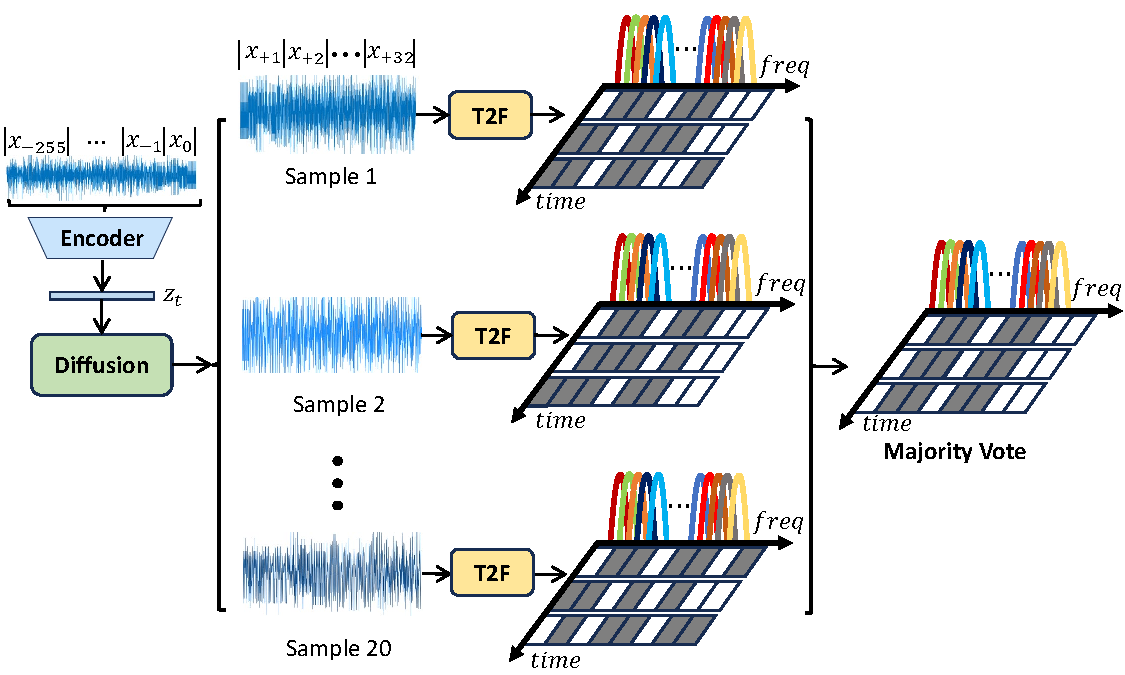
\includegraphics[width=3.5in]{Fig/Slide4.pdf}
\caption{System's Final Inference Flow: The system begins with the Encoder (LSE), which compresses the historical signal into a latent space vector $z_t$, serving as the condition for the Latent Diffusion Model. The Diffusion Model generates 20 future signals under the same latent space vector $z_t$. The CNN-based T2F model subsequently processes each generated signal to determine the frequency domain occupation for each future time frame. A majority vote is conducted for each frequency sub-block to finalize the prediction for all future time frames’ frequency sub-blocks across the generated signals.}
\label{fig_inference}
\end{figure}

The inference workflow is shown in Fig.~\ref{fig_inference}. To ensure high-fidelity outcomes and that the diffusion model's random sampling closely aligns with the ground truth regarding probability distribution, we performed 20 sampling iterations using the same context vector $z_t$. For each iteration, the T2F model was employed to predict the occupancy status of each frequency block across different time frames. A confidence threshold was then applied to the T2F model's output to finalize the spectrum situation for each iteration. This threshold was determined through ROC curve analysis at varying confidence levels, as shown in Fig. \ref{fig_res6}. The area under the ROC curve (AUC) was 0.8388, and the F1 score was 0.84. Because the T2F classifier is nearly perfect when applied to ground-truth waveforms (Fig. \ref{fig_res5}), the residual system-level error is attributable almost entirely to the generative stage — the gap between sampled futures and the realized future — identifying the diffusion model as the principal target for further accuracy improvement.

The ROC curve highlights an optimal global threshold that balances precision and recall. Applying a majority vote introduces a trade-off between inference speed and final accuracy—more sampling iterations can enhance accuracy but may slow down the overall inference process. Additionally, the diffusion model's configuration can be tailored for faster inference or improved denoising reliability, depending on the sampling method (e.g., DDIM~\cite{Song2021DDIM} or DDPM~\cite{Ho2020DDPM}), the time step size in the reverse diffusion process, and the number of time frames generated. This flexibility demonstrates the model's adaptability to various operational requirements, ensuring speed and accuracy in spectrum utilization forecasting.

\begin{figure*}[!t]
\centering
\subfloat[]{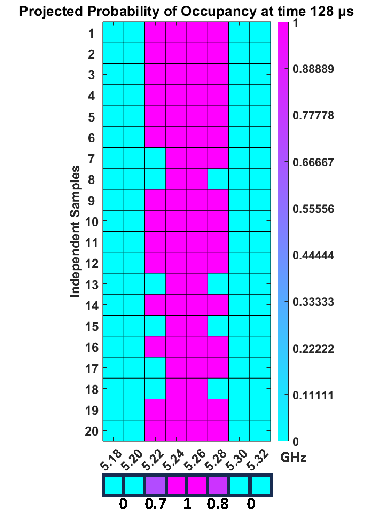
\includegraphics[width=2.3in]{Fig/Slide5a.pdf}%
\label{fig_res7}}
\hfil
\subfloat[]{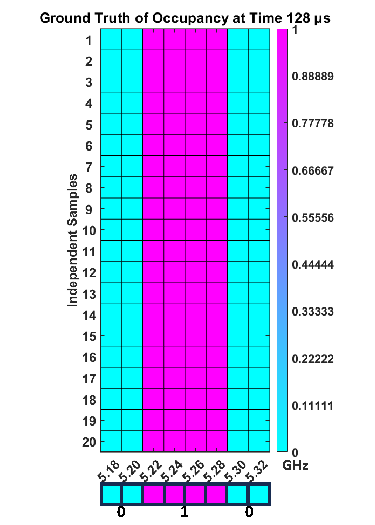
\includegraphics[width=2.3in]{Fig/Slide5b.pdf}%
\label{fig_res8}}
\vfil
\centering
\subfloat[]{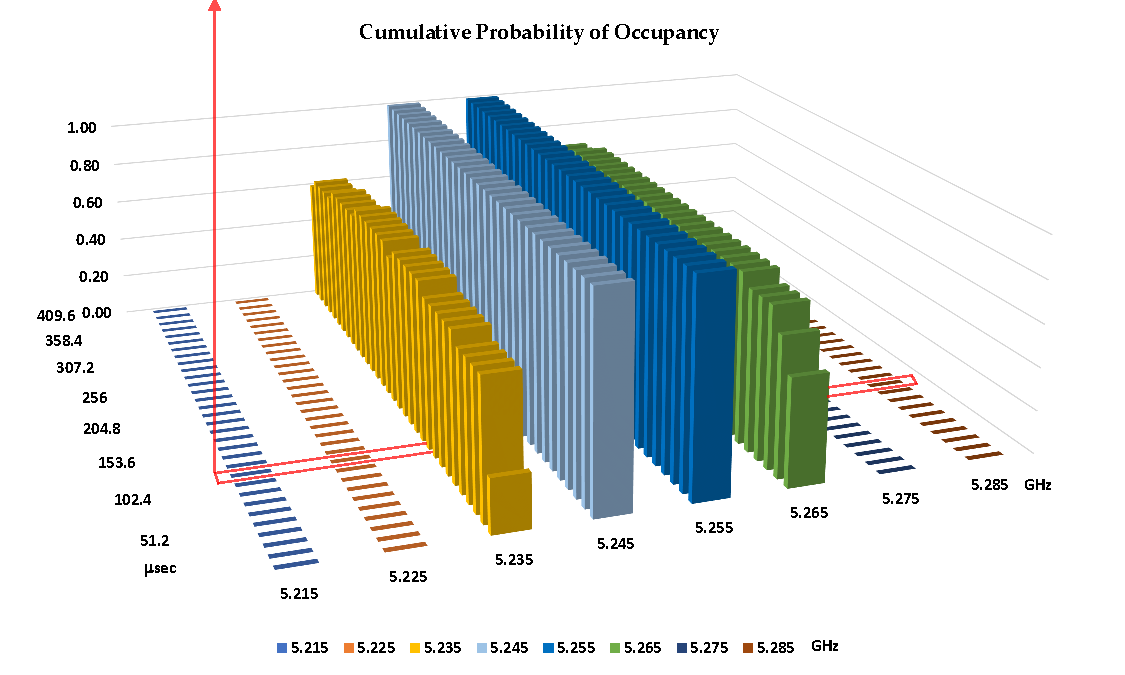
\includegraphics[width=7.5in]{Fig/Slide5c.pdf}%
\label{fig_res9}}
\caption{Future signal’s frequency occupation (a) Predicted probability of occupancy at 128 $\mu$s in the future from 20 independent diffusion model outputs with the same history waveform, (b) Ground truth at 128 $\mu$s in the future for the same history waveform, (c) Cumulative probability of occupancy with all 20 diffusion model outputs at each time step from 12.8 $\mu$s to 409.6 $\mu$s with same history signal input.}
\label{fig_result2}
\end{figure*}

Additional inference results are illustrated in Fig. \ref{fig_result2}, where spectrum occupation changes during the prediction period. The results confirm that the entire spectrum prediction model successfully interprets meaningful information from the historical data. The diffusion model accurately predicts when current users will end their communication in the prediction time and when new potential users will enter the communication system.

Our model provides frame-by-frame predictions, in contrast to previous models, which rely on power information or matched filter detection and can only predict spectrum occupancy over extended time ranges. This granularity enables precise identification of user communication patterns and transitions. Furthermore, by combining the diffusion model with the history encoder, our approach can accurately determine the end of current communications and the onset of new ones, showcasing a deeper understanding of each user's communication content and significantly enhancing real-time spectrum management capabilities.

We compare our work with previous AI-based spectrum prediction methods in Table \ref{tab:compare1} and find that previous approaches suffer from low time or frequency resolution, limited ability to model dynamic user behavior, and an inability to predict events such as users leaving or joining a communication channel. In contrast, our model effectively addresses these issues, offering predictions across multiple time slots with high temporal and frequency granularity. Using signal waveforms as input, our approach successfully captures the probabilistic features of queue networks, enabling precise modeling of user transitions. 

\begin{table*}[ht]
\centering
\caption{Stage ablations. Every row is evaluated on the same validation draw (60 windows per environment, seed 42, $N{=}1800$) over the 32-frame horizon, scoring each sub-block by the sample-averaged classifier confidence. AP is average precision; its no-skill floor equals the occupied-class base rate of 0.777. Vacancy det.\ @ 1\% collision is the fraction of genuinely vacant sub-blocks identified when the decision threshold is set so that 1\% of occupied sub-blocks are declared vacant. Latency is the median single-inference wall clock on one NVIDIA A100; the direct-regression head is a 4.7M-parameter network on the frozen encoder context. Under this common protocol the full system measures an AUC of 0.7612 and the zero-shot configuration 0.7491; these differ from the values quoted in Sections~\ref{sec:sys_eval} and~\ref{sec:zeroshot}, whose original evaluation windows are not recoverable. The persistence baseline saturates because occupancy dwell times far exceed the 410~$\mu$s prediction horizon.}
\label{tab:comparison}
\resizebox{\textwidth}{!}{%
\begin{tabular}{|p{3.2cm}|p{1.8cm}|p{1.2cm}|p{1.2cm}|p{2.8cm}|p{2.5cm}|}
\hline
\textbf{Configuration} & \textbf{Generative stage} & \textbf{AUC} & \textbf{AP} & \textbf{Vacancy det. @ 1\% collision} & \textbf{Latency / inference} \\
\hline

Persistence (repeat frame 0)
  & \textit{none} & 1.0000 & 1.0000 & 100.0\% & $<1$ $\mu$s \\
\hline

Encoder $\rightarrow$ CNN, direct label regression
  & \textit{removed} & 0.7789 & 0.9295 & 3.2\% & 19.5 \ul{ms} \\
\hline

Encoder $\rightarrow$ diffusion $\rightarrow$ T2F, 1 sample
  & full & 0.7449 & 0.9204 & 1.8\% & 457 \ul{ms} \\
\hline

Encoder $\rightarrow$ diffusion $\rightarrow$ T2F, 5 samples
  & full & 0.7570 & 0.9200 & 2.1\% & 1979 \ul{ms} \\
\hline

\textbf{Proposed (20 samples, ensemble mean)}
  & \textbf{full} & \textbf{0.7612} & \textbf{0.9250} & \textbf{1.8\%} & \textbf{8025 \ul{ms}} \\
\hline

Proposed, zero-shot (Sec. V-E)
  & full & 0.7491 & 0.9169 & 1.8\% & 8079 \ul{ms} \\
\hline

\textit{T2F on ground-truth waveforms (upper bound)}
  & \textit{oracle} & \textit{0.9855} & \textit{0.9780} & \textit{98.3\%} & --- \\
\hline

\end{tabular}%
}
\end{table*}




\begin{table}[ht]
\centering
\caption{Design-choice ablations on the saved system checkpoint. Each row varies one inference-time element; the AUC column reports the varied setting and $\Delta$~AUC is relative to the proposed configuration (0.7612) under the protocol of Table~\ref{tab:comparison}. The fixed-threshold majority vote is degenerate at this operating point — nearly every per-sample confidence exceeds 0.5 — so threshold-free ranking requires the ensemble-mean confidence or a swept vote threshold as in Fig.~\ref{fig_res6}.}
\label{tab:ablation}
\begin{tabular}{|>{\centering\arraybackslash}m{1.8cm}|>{\centering\arraybackslash}m{2.8cm}|>{\centering\arraybackslash}m{1.0cm}|>{\centering\arraybackslash}m{1.2cm}|}
\hline
\textbf{Ablation} & \textbf{Setting compared} & \textbf{AUC} & \textbf{$\Delta$ AUC} \\
\hline

Sampler
  & DDPM vs. DDIM (10 steps each) & 0.7711 & $+0.0099$ \\
\hline

Ensemble aggregation
  & mean probability vs. majority vote (fixed 0.5) & 0.5000 & $-0.2612$ \\
\hline

\end{tabular}
\end{table}







\begin{table*}[!t]
\centering
\caption{Comparison with other works $^1$
\label{tab:compare1}}
\begin{tabular}{|c|c|c|c|c|c|c|c|c|}
\hline
Work & Method & \makecell{Input Format} & \makecell{Historical\\ Duration} & \makecell{Number \\of\\ Predicted \\ Time Slots} & \makecell{Interval \\(s)} & \makecell{Frequency \\Span} & \makecell{Frequency \\ block(s)} & \makecell{Dynamic \\ Prediction} \\
\hline

\cite{intro_ref7} & ConvLSTM & \makecell{Signal Power \\ $[S \times f$, $t]^2$ } & \makecell{Weekly + \\ Daily + \\ minutes} & $\leq$ 6 & \makecell{10 mins} & \makecell{790 MHz -\\ 850 MHz} & 60 & \xmark \\
\hline

\cite{intro_ref12} & RNN & \makecell{Duty Cycle \\(Signal Power) \\ $[1, t]$} & $\sim$ 2 ms & 1 & 0.8 ms & \makecell{2.436 GHz -\\ 2.437 GHz} & 1 & \xmark \\
\hline

\cite{intro_ref20} & RNN & \makecell{Channel State \\(0/1 labels) \\ $[f, t]$} & 1 s & 1 & 0.1 s & \makecell{390 MHz -\\ 490 MHz} & 5120 & \xmark \\
\hline

\makecell{This work} & Generative Model & \makecell{\textbf{Raw} \\ \textbf{Signal Waveform} \\ $[1, t]$} & 819 $\mu$s & \textbf{32} & \textbf{12.8} $\mu$s & \makecell{5.2 GHz -\\ 5.3 GHz} & 8 & \cmark \\
\hline

\multicolumn{9}{l}{\makecell[l]{$^1$ The comparison is based on reported results in the respective publications and the experimental datasets are different.}} \\

\multicolumn{9}{l}{\makecell[l]{$^2$ $[S \times f$, $t]$ indicates the data is in a 2D matrix (Space $\times$ Frequency), sampled at different time points and stacking together among time domain. }}

\end{tabular}
\end{table*}

\subsection{Zero-Shot Transfer to Unseen Environments}\label{sec:zeroshot}

The system-level results reported above draw the training and validation data from the same 30 simulated environments. To examine how the framework behaves when the diffusion model encounters wireless environments that were never part of its training set, we retrain the diffusion model using only environments 1--20 and hold out environments 21--30 entirely. The architecture, diffusion schedule, and training configuration are identical to those of the original model. The encoder and the T2F model are reused unchanged from the full-training configuration, so that this experiment isolates the transfer behavior of the diffusion model.

Evaluation on the ten held-out environments follows the same inference procedure as Fig.~\ref{fig_inference} and the same ROC methodology as Fig.~\ref{fig_res6}: for each input history, 20 future signals are sampled under the same latent space vector $z_t$, each generated signal is classified by the T2F model, a majority vote across the samples finalizes the occupancy decision for each frequency sub-block, and the ROC curve is traced by sweeping the confidence threshold. Table~\ref{tab:zeroshot} lists the resulting AUC for each held-out environment. The system attains an overall AUC of 0.7589 on environments never seen by the diffusion model, compared with 0.8388 when all 30 environments are included in training (Section~\ref{sec:sys_eval}), and the F1 score at the fixed 0.5 threshold is 0.87. As in the main evaluation, the held-out environments are simulated channel realizations drawn under the same traffic model, and the transfer result should be interpreted within that scope.

The moderate reduction in AUC indicates that a substantial portion of the system-level sub-channel occupancy classification performance is retained when the diffusion model operates outside its training distribution. This behavior is consistent with the cross-environment generalization goal of the contrastive representation discussed at the beginning of this section. Few-shot adaptation of the encoder and the T2F model to new environments remains a natural extension for future work.

\begin{table}[!t]
\centering
\caption{Zero-Shot System-Level AUC on Held-Out Environments
\label{tab:zeroshot}}
\begin{tabular}{cc|cc}
\hline
Environment & AUC & Environment & AUC \\
\hline
21 & 0.7188 & 26 & 0.6762 \\
22 & 0.8244 & 27 & 0.8982 \\
23 & 0.7171 & 28 & 0.7400 \\
24 & 0.7595 & 29 & 0.8048 \\
25 & 0.8179 & 30 & 0.7371 \\
\hline
\multicolumn{2}{c|}{Overall} & \multicolumn{2}{c}{\textbf{0.7589}} \\
\hline
\end{tabular}
\end{table}

\section{Discussion}
The central contribution of this work is enabling devices that traditionally require separate frequency bands — such as radar, satellite links, and IoT sensors — to coexist within the same band as WiFi by exploiting subchannel-level vacancies in real time.

The key enabler is temporal resolution. By predicting occupancy at the individual OFDM frame level (approximately 13~$\mu$s), the model can in principle anticipate subchannel availability before a WiFi transmission ends. Practical deployment, however, requires that the end-to-end inference pipeline — including encoder, diffusion sampling, and T2F classification — completes within this time budget, which has not yet been demonstrated on embedded hardware and represents an important avenue for future work. This allows secondary devices to begin transmitting in vacant subchannels almost immediately, rather than waiting for the entire band to be released and reassigned — directly reducing idle spectrum and increasing overall spectral efficiency. This anticipatory capability fundamentally distinguishes our approach from conventional spectrum sensing, which can only observe current conditions.

The diffusion model's probabilistic nature is well suited to this task because user arrivals and departures are inherently stochastic. Rather than producing a single deterministic forecast, the model generates multiple plausible future signals and aggregates them via majority voting, yielding predictions that are robust to the uncertainty of real-world spectrum dynamics. The contrastive-learning-based encoder is designed to generalize across diverse wireless environments by learning environment-agnostic representations. In this work, generalization is evaluated across the 30 simulated scenarios; transfer to real-world deployments with hardware impairments, unknown interference sources, or different air interface standards remains to be validated.

From a spectral efficiency standpoint, resolving occupancy down to eight 10 MHz sub-blocks within an 80 MHz band reveals sharing opportunities invisible to full-band methods. A secondary user does not need an entire band to be free — only a few unoccupied subchannels that can be identified and accessed quickly enough to avoid collision with WiFi. This granularity is what makes true simultaneous coexistence feasible.

The system's inference process involves a configurable trade-off between speed and accuracy through the number of diffusion samples and reverse steps, allowing adaptation to different operational requirements. While validated here through IEEE 802.11ax simulations, the framework is not inherently limited to WiFi and could be extended to other standards, broader frequency ranges, and real-world deployments in future work.

\section{Applicability to Other Use-Cases}\label{sec:other_use_cases}

While this paper largely focuses on spectrum prediction at the OFDM frame level, the model can be adapted for other use cases. Here, we present an experimental example predicting spectrum occupancy for a stream of Wi-Fi packets without distinguishing between individual OFDM frames within the packet.

The experimental setup consists of two National Instruments (NI) USRP X310 software-defined radios (SDRs) connected to independent computers with 10 GbE networking to support the high-bandwidth Wi-Fi packets. Both USRPs use UBX-160 daughter boards and 5.1-5.9 GHz Blade antennas. Radio control, packet transmission, and reception are performed in MATLAB 2025a with the appropriate USRP toolboxes. The receiving USRP uses a modified version of the software available at \cite{mathworks2025recover} for over-the-air packet identification and segmentation.

Using the approach from Section~\ref{sec:data}, we generated three 5-second base scenarios under ideal conditions (i.e., without AWGN or channel impairments). Each base scenario produced an average of 1200 packets with an idle time of 30~$\mu$s between them. These packets were then transmitted over the air to create the final dataset. For each 5-second transmission, representing a single scenario with a fixed channel condition, the $\approx$ 1200 packets were sent sequentially in batches of 3-6 due to computer memory limitations.

\begin{figure}[!t]
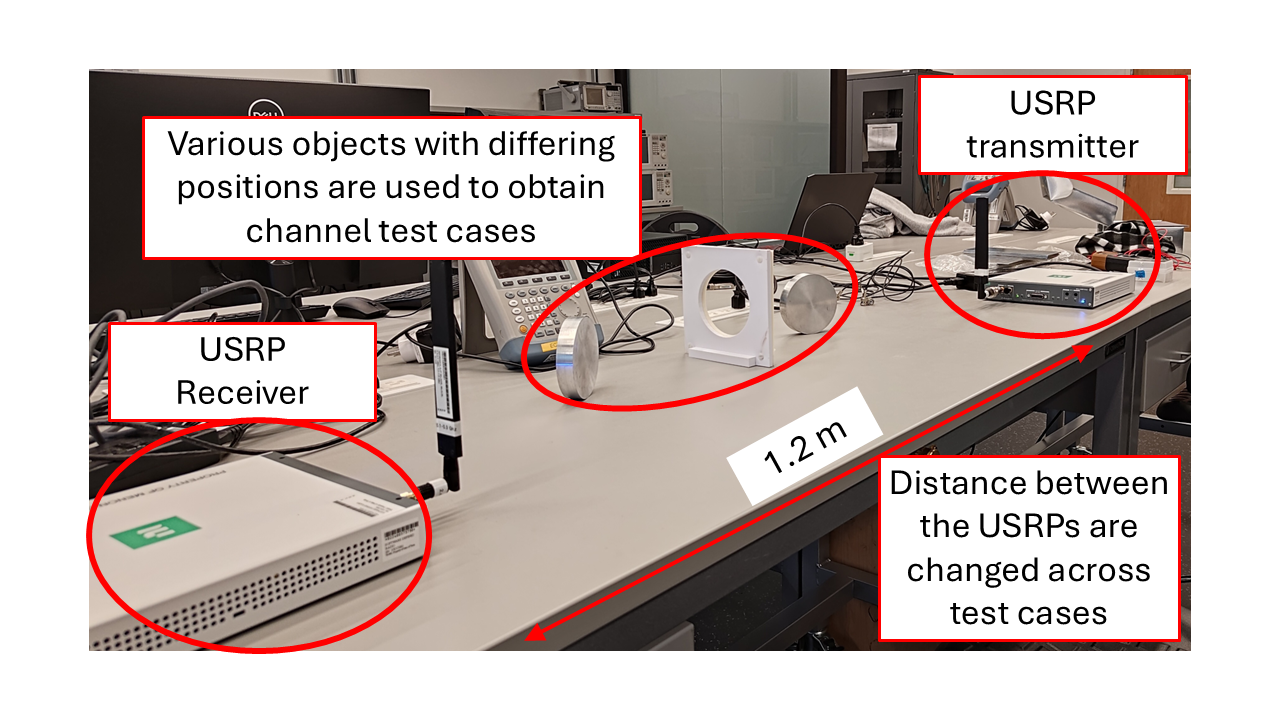
\includegraphics[width=3.4in]{Fig/measurement_setup.png}
\caption{An example Wi-Fi transmit-receive link created using NI USRP X310 software defined radios.}
\label{fig_meas_SDR}
\end{figure}

We created the various channel test cases by modifying the distance between the USRPs (2-4 ft), placing metallic and dielectric objects and fans around the SDRs, and, in one case, inserting a plywood barrier between them. The setup was placed in a typical lab environment, with a typical setup shown in Fig.~\ref{fig_meas_SDR}, which included interference from nearby Wi-Fi devices and routers. To ensure data integrity, successful reception was defined by an Error Vector Magnitude (EVM) threshold of $-10$~dB; for comparison, typical packets demonstrated an EVM of $-30$~dB.

The received recordings form a packet-level dataset: each packet is stored as complex baseband IQ samples at an 80~MHz sampling rate and is annotated with the ground-truth occupancy of the eight 10~MHz frequency sub-blocks, and the recordings under three channel test conditions, comprising 1202 packets each, serve as three distinct environments. For processing, each packet is resampled to 2048 samples, and the prediction unit becomes an individual packet rather than a fixed-duration OFDM frame: the system observes 128 consecutive packets and predicts the sub-block occupancy of the following 32 packets.

All three components are retrained on this dataset with unchanged architectures. The encoder is retrained with the same contrastive objective, with in-batch negatives drawn across the three channel test conditions; the T2F classifier is retrained on ground-truth waveforms, where it again attains near-perfect classification accuracy; and the diffusion model is retrained conditioned on the resulting latent space vector $z_t$. The three components are then jointly fine-tuned for six epochs following the procedure of Section~\ref{sec:methods}. Inference mirrors Fig.~\ref{fig_inference}: for each input history, 20 future signals are sampled under the same latent space vector $z_t$, each generated signal is classified by the T2F model, and the classifier outputs are averaged over the 20 samples and thresholded at 0.5 — an ensemble-mean variant of the majority vote used in Section~\ref{sec:sys_eval}. Under this protocol, sub-block occupancy accuracy rises from 0.772 after the first fine-tuning epoch to a best value of 0.828 with an F1 score of 0.899, while the normalized ADE and FDE converge to 0.059.

Two qualifications bound the scope of this result. First, the packet-window sampler in this configuration draws training and evaluation windows from the same pool, so the reported figures characterize in-sample fit on the recorded dataset rather than held-out generalization; generalization to unseen environments is instead assessed on the simulated corpus in Section~\ref{sec:zeroshot}. Second, no ROC analysis is reported for this dataset. Within this scope, the experiment demonstrates that the complete framework — the contrastive encoder, the conditional diffusion model, and the T2F classifier — trains stably end-to-end on packet-level over-the-air recordings and reproduces their sub-block occupancy structure at accuracy levels comparable to the simulation-based system evaluation of Section~\ref{sec:sys_eval}.

\section{Conclusion}
This paper presents a deep neural network framework that enables simultaneous spectrum sharing between WiFi and other devices or signal types — such as radar, satellite communications, and IoT sensors — within the same frequency band. By predicting which subchannels are vacant at any given moment, the system allows secondary users to transmit in those gaps without interfering with ongoing WiFi communications, directly reducing spectrum congestion and increasing spectral efficiency. The framework combines a contrastive-learning-based encoder for cross-environment generalization, a probabilistic diffusion model for realistic future signal generation, and a CNN-based classifier for subchannel-level occupancy prediction — all operating at the resolution of individual OFDM frames (approximately 13~$\mu$s), far exceeding the granularity of prior methods. Validated across 30 simulated environments under the IEEE 802.11ax standard, the model predicts 32 future frames with a normalized ADE of 0.047 and a system-level AUC of 0.84. These results establish the feasibility of AI-driven sub-channel-level prediction at microsecond resolution, and identify real-world hardware validation, longer-horizon prediction, and extension to heterogeneous air interface standards as the principal directions for future investigation. As wireless demand continues to outpace new frequency allocations, frameworks like this will be essential for enabling dense coexistence of diverse wireless systems within shared bands.



% {\appendix[Proof of the Zonklar Equations]
% Use $\backslash${\tt{appendix}} if you have a single appendix:
% Do not use $\backslash${\tt{section}} anymore after $\backslash${\tt{appendix}}, only $\backslash${\tt{section*}}.
% If you have multiple appendixes use $\backslash${\tt{appendices}} then use $\backslash${\tt{section}} to start each appendix.
% You must declare a $\backslash${\tt{section}} before using any $\backslash${\tt{subsection}} or using $\backslash${\tt{label}} ($\backslash${\tt{appendices}} by itself
%  starts a section numbered zero.)}



%{\appendices
%\section*{Proof of the First Zonklar Equation}
%Appendix one text goes here.
% You can choose not to have a title for an appendix if you want by leaving the argument blank
%\section*{Proof of the Second Zonklar Equation}
%Appendix two text goes here.}



% \section{References Section}
% You can use a bibliography generated by BibTeX as a .bbl file.
%  BibTeX documentation can be easily obtained at:
%  http://mirror.ctan.org/biblio/bibtex/contrib/doc/
%  The IEEEtran BibTeX style support page is:
%  http://www.michaelshell.org/tex/ieeetran/bibtex/
 
 % argument is your BibTeX string definitions and bibliography database(s)
%\bibliography{IEEEabrv,../bib/paper}
%
% \section{Simple References}
% You can manually copy in the resultant .bbl file and set second argument of $\backslash${\tt{begin}} to the number of references
%  (used to reserve space for the reference number labels box).

\section*{Acknowledgment}
The authors would like to thank the Intelligent Electromagnetic Sensor Laboratories (iEMSL) at Texas A\&M University for providing access to facilities and resources that supported this research. The authors also wish to thank Mr. Yi Huang at the University of Massachusetts, Amherst, for providing critical comments during the development of this manuscript as well as Sanjay Patel and Mariea Sharaf Anzum of Texas A\&M University for their assistance with measurements. The authors received no external funding for this work.

\begin{thebibliography}{1}
\bibliographystyle{IEEEtran}

\bibitem{intro_ref1}
Azmat, Freeha \& Chen, Yunfei \& Stocks, Nigel. (2015), ``Analysis of Spectrum Occupancy Using Machine Learning Algorithms,'' \textit{IEEE Transactions on Vehicular Technology}, 65. 10.1109/TVT.2015.2487047.

\bibitem{intro_ref2}
Rahman, Aniq Ur, Mustafa A. Kishk, and Mohamed-Slim Alouini, ``Improving Spectral Efficiency of Wireless Networks through Democratic Spectrum Sharing,'' \textit{arXiv preprint}, arXiv:2111.10570 (2021)

\bibitem{intro_ref3}
Md Jalil Piran, Quoc-Viet Pham, S.M. Riazul Islam, Sukhee Cho, Byungjun Bae, Doug Young Suh, Zhu Han, ``Multimedia communication over cognitive radio networks from QoS/QoE perspective: A comprehensive survey,'' \textit{Journal of Network and Computer Applications}, Volume 172, 2020, 102759, ISSN 1084-8045, https://doi.org/10.1016/j.jnca.2020.102759

\bibitem{intro_ref4}
M. Chen, A. Liu, W. Liu, K. Ota, M. Dong and N. N. Xiong, ``RDRL: A Recurrent Deep Reinforcement Learning Scheme for Dynamic Spectrum Access in Reconfigurable Wireless Networks,'' \textit{IEEE Transactions on Network Science and Engineering}, vol. 9, no. 2, pp. 364-376, 1 March-April 2022, doi: 10.1109/TNSE.2021.3117565

\bibitem{intro_ref5}
Emmert-Streib, Frank, et al, ``An introductory review of deep learning for prediction models with big data,'' \textit{Frontiers in Artificial Intelligence}, 3 (2020): 4.

\bibitem{intro_ref6}
Young, Tom, et al, ``Recent trends in deep learning based natural language processing,'' \textit{IEEE Computational Intelligence Magazine}, 13.3 (2018): 55-75

\bibitem{intro_ref7}
X. Li, Z. Liu, G. Chen, Y. Xu and T. Song, ``Deep Learning for Spectrum Prediction From Spatial–Temporal–Spectral Data,'' \textit{IEEE Communications Letters}, vol. 25, no. 4, pp. 1216-1220, April 2021, doi: 10.1109/LCOMM.2020.3045205

\bibitem{intro_ref8}
Ren, Xiangyu, et al, ``Spatio-temporal spectrum load prediction using convolutional neural network and ResNet,'' \textit{IEEE Transactions on Cognitive Communications and Networking}, 8.2 (2021): 502-513

\bibitem{intro_ref9}
Ren, Xiangyu, et al, ``Spatio-temporal spectrum load prediction using convolutional neural network and Bayesian estimation,'' \textit{GLOBECOM 2020-2020 IEEE Global Communications Conference}, IEEE, 2020.

\bibitem{intro_ref10}
Huang, Jiaxing, et al, ``Model adaptation: Historical contrastive learning for unsupervised domain adaptation without source data.,'' \textit{Advances in Neural Information Processing Systems }, 34 (2021): 3635-3649

\bibitem{intro_ref11}
Fujieda, Shin, Kohei Takayama, and Toshiya Hachisuka, ``Wavelet convolutional neural networks,'' \textit{arXiv preprint}, arXiv:1805.08620 (2018)

\bibitem{intro_ref12}
Umebayashi, Kenta, et al, ``Spectrum Occupancy Prediction based on adaptive Recurrent Neural Networks,'' \textit{2023 IEEE Wireless Communications and Networking Conference (WCNC)}, IEEE, 2023

\bibitem{intro_ref13}
Suriya, M, ``Study of Spectrum Prediction Techniques in Cognitive Radio Networks,'' \textit{2022 8th International Conference on Advanced Computing and Communication Systems (ICACCS)}, Vol. 1. IEEE, 2022

\bibitem{intro_ref14}
Wu, Jianwei, and Yanling Li, ``A survey of spectrum prediction methods in cognitive radio networks,'' \textit{AIP Conference Proceedings}, Vol. 1834. No. 1. AIP Publishing, 2017

\bibitem{intro_ref15}
TIDJANI, Sayhia, and Zoheir HAMMOUDI, ``A survey on spectrum prediction methods in cognitive radio networks,'' \textit{International Journal of Computing}, 8.2 (2019): 24-31

\bibitem{intro_ref17}
Eltom, Hamid, et al, ``Statistical spectrum occupancy prediction for dynamic spectrum access: a classification,'' \textit{EURASIP Journal on Wireless Communications and Networking 2018}, (2018): 1-17.

\bibitem{intro_ref18}
Ko{\c{c}}kaya, Kenan, and Ibrahim Develi, ``Spectrum sensing in cognitive radio networks: threshold optimization and analysis,'' \textit{EURASIP Journal on Wireless Communications and Networking 2020.1}, (2020): 255

\bibitem{intro_ref19}
J. Adu Ansere, G. Han, H. Wang, C. Choi and C. Wu, ``A Reliable Energy Efficient Dynamic Spectrum Sensing for Cognitive Radio IoT Networks,'' \textit{IEEE Internet of Things Journal}, vol. 6, no. 4, pp. 6748-6759, Aug. 2019, doi: 10.1109/JIOT.2019.2911109

\bibitem{intro_ref20}
D. S. Chirov and E. O. Kandaurova, ``Spectrum Occupancy Prediction Algorithm Using Artificial Neural Networks,'' \textit{2023 Systems of Signals Generating and Processing in the Field of on Board Communications}, Moscow, Russian Federation, 2023, pp. 1-4

\bibitem{Yucek_2009}
Yucek, T. and Arslan, H. A survey of spectrum sensing algorithms for cognitive radio applications. {\em IEEE Communications Surveys \& Tutorials}. \textbf{11}, 116-130 (2009)

\bibitem{He_2010}
He, A., Bae, K., Newman, T., Gaeddert, J., Kim, K., Menon, R., Morales-Tirado, L., Neel, J., Zhao, Y., Reed, J. \& Tranter, W. A Survey of Artificial Intelligence for Cognitive Radios. {\em IEEE Transactions On Vehicular Technology}. \textbf{59}, 1578-1592 (2010)

\bibitem{Xing_2013}Xing, X., Jing, T., Cheng, W., Huo, Y. \& Cheng, X. Spectrum prediction in cognitive radio networks. {\em IEEE Wireless Communications}. \textbf{20}, 90-96 (2013)

\bibitem{Chen_2016}Chen, Y. \& Oh, H. A Survey of Measurement-Based Spectrum Occupancy Modeling for Cognitive Radios. {\em Commun. Surveys Tuts.}. \textbf{18}, 848-859 (2016,1), https://doi.org/10.1109/COMST.2014.2364316

\bibitem{Ding_2017}Ding, G., Jiao, Y., Wang, J., Zou, Y., Wu, Q., Yao, Y. \& Hanzo, L. Spectrum Inference in Cognitive Radio Networks: Algorithms and Applications. {\em IEEE Communications Surveys \& Tutorials}. \textbf{20}, 150-182 (2018)

\bibitem{Wang_2024}Wang, L., Hu, J., Zhang, C., Jiang, R. \& Chen, Z. Deep Learning Models for Spectrum Prediction: A Review. {\em IEEE Sensors Journal}. \textbf{24}, 28553-28575 (2024)


\bibitem{Raouf_2023}Raouf, A., Maeng, S., Guvenc, I., {\"O}zdemir, {\"O}. \& Sichitiu, M. Cellular Spectrum Occupancy Probability in Urban and Rural Scenarios at Various UAS Altitudes. {\em 2023 IEEE 34th Annual International Symposium On Personal, Indoor And Mobile Radio Communications (PIMRC)}. pp. 1-6 (2023)

\bibitem{Wellens_2007}Wellens, M., Wu, J. \& Mahonen, P. Evaluation of Spectrum Occupancy in Indoor and Outdoor Scenario in the Context of Cognitive Radio. {\em 2007 2nd International Conference On Cognitive Radio Oriented Wireless Networks And Communications}. pp. 420-427 (2007)

\bibitem{Engiz_2021}Engiz, B. \& Rajab, Y. Spectrum occupancy measurements in cellular frequency band in Samsun. {\em Balkan Journal Of Electrical And Computer Engineering}. \textbf{9}, 138-143 (2021)

\bibitem{Kozlowski_2021}Koz{\l}owski, S. \& Kurek, K. Channel occupancy measurements in 868 mhz ism band in residential areas. {\em Sensors}. \textbf{21}, 7805 (2021)


\bibitem{Muzaffar_2024}Muzaffar, M. \& Sharqi, R. A review of spectrum sensing in modern cognitive radio networks. {\em Telecommunication Systems}. \textbf{85}, 347-363 (2024)

\bibitem{Segura_2010}Font-Segura, J. \& Wang, X. GLRT-based spectrum sensing for cognitive radio with prior information. {\em Trans. Comm.}. \textbf{58}, 2137-2146 (2010,7), https://doi.org/10.1109/TCOMM.2010.07.090556

\bibitem{Tian_2006}Tian, Z. \& Giannakis, G. A Wavelet Approach to Wideband Spectrum Sensing for Cognitive Radios. {\em 2006 1st International Conference On Cognitive Radio Oriented Wireless Networks And Communications}. pp. 1-5 (2006)

\bibitem{Wellens_2010}Wellens, M. \& M{\"a}h{\"o}nen, P. Lessons learned from an extensive spectrum occupancy measurement campaign and a stochastic duty cycle model. {\em Mobile Networks And Applications}. \textbf{15}, 461-474 (2010)

\bibitem{Gibson_1994}Gibson, A. \& Arnett, L. Measurements and statistical modelling of spectrum occupancy. {\em Sixth International Conference On HF Radio Systems And Techniques}. pp. 150-154 (1994)

\bibitem{Percival_1997}Percival, D., Kraetzl, M. \& Britton, M. A Markov model for HF spectral occupancy in central Australia. {\em Seventh International Conference On HF Radio Systems And Techniques}. pp. 14-18 (1997)

\bibitem{Chen_2011}Chen, Z., Guo, N., Hu, Z. \& Qiu, R. Channel state prediction in cognitive radio, Part II: Single-user prediction. {\em 2011 Proceedings Of IEEE Southeastcon}. pp. 50-54 (2011)

\bibitem{Akbar_2007}Akbar, I. \& Tranter, W. Dynamic spectrum allocation in cognitive radio using hidden Markov models: Poisson distributed case. {\em Proceedings 2007 IEEE SoutheastCon}. pp. 196-201 (2007)

\bibitem{Saad_2016}Saad, A., Staehle, B. \& Knorr, R. Spectrum prediction using hidden Markov models for industrial cognitive radio. {\em 2016 IEEE 12th International Conference On Wireless And Mobile Computing, Networking And Communications (WiMob)}. pp. 1-7 (2016)

\bibitem{Xing_2013_channel_qual}Xing, X., Jing, T., Huo, Y., Li, H. \& Cheng, X. Channel quality prediction based on Bayesian inference in cognitive radio networks. {\em 2013 Proceedings IEEE INFOCOM}. pp. 1465-1473 (2013)

\bibitem{Pan_2026}Pan, G., Yau, D., Zhou, B. \& Wu, Q. Deep Learning for Spectrum Prediction in Cognitive Radio Networks: State-of-the-Art, New Opportunities, and Challenges. {\em IEEE Network}. \textbf{40}, 192-200 (2026)

\bibitem{Yule_1927}Yule, G. On a Method of Investigating Periodicities in Disturbed Series, with Special Reference to Wolfer's Sunspot Numbers. {\em Philosophical Transactions Of The Royal Society A}. \textbf{226} pp. 267-298 (1927)

\bibitem{Slutzky1937Summation}Slutsky, E. Summation of random causes as the source of cyclic processes. {\em Econometrica}. \textbf{5} pp. 105-146 (1937)

\bibitem{Box_1978}Box, G., Jenkins, G., Reinsel, G. \& Ljung, G. Time Series Analysis: Forecasting and Control. {\em The Statistician}. \textbf{27} pp. 265-265 (1978)

\bibitem{Hou_2021}Hou, Y., Webber, J., Yano, K., Kawasaki, S., Denno, S. \& Suzuki, Y. Modeling and Predictability Analysis on Channel Spectrum Status Over Heavy Wireless LAN Traffic Environment. {\em IEEE Access}. \textbf{9} pp. 85795-85812 (2021)

\bibitem{Su_2009}Su, J. \& Wu, W. Wireless spectrum prediction model based on time series analysis method. {\em Proceedings Of The 2009 ACM Workshop On Cognitive Radio Networks}. pp. 61-66 (2009), https://doi.org/10.1145/1614235.1614250

\bibitem{Tabassam_2011}Tabassam, A., Suleman, M., Khan, S. \& Tirmazi, S. Spectrum estimation and spectrum hole opportunities prediction for cognitive radios using higher-order statistics. {\em 2011 Wireless Advanced}. pp. 213-217 (2011)

\bibitem{Pedraza_2016}Pedraza, L., Suarez, C., Paez, I., Trivino, J. \& Rodr{\'\i}guez-Colina, E. Linear Algorithms for Radioelectric Spectrum Forecast. {\em Algorithms}. \textbf{9} pp. 82 (2016)

\bibitem{Tumuluru_2010}Tumuluru, V., Wang, P. \& Niyato, D. A Neural Network Based Spectrum Prediction Scheme for Cognitive Radio. {\em 2010 IEEE International Conference On Communications}. pp. 1-5 (2010)

\bibitem{Yin_2011}Yin, L., Yin, S., Hong, W. \& Li, S. Spectrum behavior learning in Cognitive Radio based on artificial neural network. {\em 2011 - MILCOM 2011 Military Communications Conference}. pp. 25-30 (2011)

\bibitem{Winston_2013}Winston, O., Thomas, A. \& OkelloOdongo, W. Optimizing Neural Network for TV Idle Channel Prediction in Cognitive Radio Using Particle Swarm Optimization. {\em 2013 Fifth International Conference On Computational Intelligence, Communication Systems And Networks}. pp. 25-29 (2013)

\bibitem{Yang_2014}Yang, L., Lv, N. \& Xu, Z. Spectrum prediction for cognitive radio system based on optimally pruned extreme learning machine. {\em Applied Mechanics And Materials}. \textbf{536} pp. 430-436 (2014)

\bibitem{Taj_2011}Taj, M. \& Akil, M. Cognitive Radio Spectrum Evolution Prediction using Artificial Neural Networks based Multivariate Time Series Modelling. {\em 17th European Wireless 2011 - Sustainable Wireless Technologies}. pp. 1-6 (2011)

\bibitem{Yang_2013}Yang, L., Liang, X., Ma, T. \& Liu, K. Spectrum Prediction Based on Echo State Network and Its Improved Form. {\em 2013 5th International Conference On Intelligent Human-Machine Systems And Cybernetics}. \textbf{1} pp. 172-176 (2013)

\bibitem{Golestanian_2014}Golestanian, M., Iranmanesh, S., Ghazizadeh, R. \& Azimi, M. A learning automata based spectrum prediction technique for cognitive radio networks. {\em International Transaction Of Electrical And Computer Engineers System}. \textbf{2}, 93-97 (2014)

\bibitem{Ni_2011}Ni, S. \& Shen, S. Frequency spectrum access mechanism of cognitive radio based on spectrum prediction. {\em IET International Conference On Communication Technology And Application (ICCTA 2011)}. pp. 556-560 (2011)

\bibitem{Wang_2017}Wang, J., Tang, J., Xu, Z., Wang, Y., Xue, G., Zhang, X. \& Yang, D. Spatiotemporal modeling and prediction in cellular networks: A big data enabled deep learning approach. {\em IEEE INFOCOM 2017 - IEEE Conference On Computer Communications}. pp. 1-9 (2017)

\bibitem{Ozyegen_2020}Ozyegen, O., Mohammadjafari, S., Kavurmacioglu, E., Maidens, J. \& Bener, A. Experimental Results on the Impact of Memory in Neural Networks for Spectrum Prediction in Land Mobile Radio Bands. {\em IEEE Transactions On Cognitive Communications And Networking}. \textbf{6}, 771-782 (2020)

\bibitem{Jia_2020}Jia, M., Zhang, X., Sun, J., Gu, X. \& Guo, Q. Intelligent Resource Management for Satellite and Terrestrial Spectrum Shared Networking toward B5G. {\em IEEE Wireless Communications}. \textbf{27}, 54-61 (2020)

\bibitem{Yu_2018}Yu, L., Chen, J., Zhang, Y., Zhou, H. \& Sun, J. Deep spectrum prediction in high frequency communication based on temporal-spectral residual network. {\em China Communications}. \textbf{15}, 25-34 (2018)

\bibitem{Zhang_2021_Accurate}Zhang, L. \& Jia, M. Accurate Spectrum Prediction Based on Joint LSTM with CNN toward Spectrum Sharing. {\em 2021 IEEE Global Communications Conference (GLOBECOM)}. pp. 1-6 (2021)

\bibitem{Ding_2020_Deep}Ding, X., Feng, L., Zou, Y. \& Zhang, G. Deep Learning Aided Spectrum Prediction for Satellite Communication Systems. {\em IEEE Transactions On Vehicular Technology}. \textbf{69} pp. 16314-16319 (2020)

\bibitem{Shawel_2019}Shawel, B., Woldegebreal, D. \& Pollin, S. Convolutional LSTM-based Long-Term Spectrum Prediction for Dynamic Spectrum Access. {\em 2019 27th European Signal Processing Conference (EUSIPCO)}. pp. 1-5 (2019)

\bibitem{Wen_2023}Wen, X., Fang, S., Xu, Z. \& Liu, H. Joint Multidimensional Pattern for Spectrum Prediction Using GNN. {\em Sensors (Basel, Switzerland)}. \textbf{23} (2023)

\bibitem{Li_2023}Li, K., Li, C., Chen, J., Zhang, Q., Liu, Z. \& He, S. Boost Spectrum Prediction With Temporal-Frequency Fusion Network via Transfer Learning. {\em IEEE Transactions On Mobile Computing}. \textbf{22}, 3209-3223 (2023)

\bibitem{Cheng_2023}Cheng, R., Zhang, J. \& others, Lightweight Spectrum Prediction Based on Knowledge Distillation. {\em Radioengineering}. \textbf{32} (2023)

\bibitem{Lin_2021}Lin, F., Chen, J., Ding, G., Jiao, Y., Sun, J. \& Wang, H. Spectrum prediction based on GAN and deep transfer learning: A cross-band data augmentation framework. {\em China Communications}. \textbf{18}, 18-32 (2021)

\bibitem{Krizhevsky_2012}Krizhevsky, A., Sutskever, I. \& Hinton, G. ImageNet Classification with Deep Convolutional Neural Networks. {\em Advances In Neural Information Processing Systems}. \textbf{25} pp. 1097-1105 (2012)
\bibitem{Vaswani_2017}Vaswani, A., Shazeer, N., Parmar, N., Uszkoreit, J., Jones, L., Gomez, A., Kaiser, {\L}. \& Polosukhin, I. Attention is all you need. {\em Advances In Neural Information Processing Systems}. \textbf{30} (2017)

\bibitem{Pan_2023}Pan, G., Wu, Q., Ding, G., Wang, W., Li, J. \& Zhou, B. An Autoformer-CSA Approach for Long-Term Spectrum Prediction. {\em IEEE Wireless Communications Letters}. \textbf{12}, 1647-1651 (2023)

\bibitem{Pan_2025}Pan, G., Yau, D., Zhou, B. \& Wu, Q. Deep Learning for Spectrum Prediction in Cognitive Radio Networks: State-of-the-Art, New Opportunities, and Challenges. {\em IEEE Network}. \textbf{40}, 192-200 (2026)

\bibitem{Ben_2025}Ben, C., Peng, Y., Wang, Y., Zhang, Q., Guo, L., Lin, Y. \& Gui, G. Enhanced Multi-Band Spectrum Prediction Using Singular Spectrum Analysis and Attention-Based BiLSTM. {\em IEEE Transactions On Cognitive Communications And Networking}. \textbf{11}, 118-126 (2025)

\bibitem{Shuang_Li_2025}Li, S., Sun, Y., Yue, W., Yao, M., Han, Y., Gui, G., Lin, Y. \& Xiang, W. A Novel Multi-Scale Time Fusion Transformer for Long-Range Spectrum Occupancy Prediction. {\em IEEE Transactions On Vehicular Technology}. \textbf{74}, 9299-9312 (2025)

\bibitem{Guan_2025}Guan, Z., Wen, W., Wu, P., Wang, C. \& Xia, M. Hybrid CNN-Transformer Based Sparse Channel Prediction for High-Mobility OTFS Systems. {\em IEEE Wireless Communications Letters}. \textbf{15} pp. 215-219 (2025)

\bibitem{Xu_2024}Xu, L., Gao, Z., Chen, Z., Wang, J., Fu, Y., Li, X., Gulliver, T. \& Le, K. Spectrum Prediction for Mobile Internet of Things Based on a DB-LSTM Algorithm. {\em IEEE Transactions On Vehicular Technology}. \textbf{73} pp. 15395-15406 (2024)




\bibitem{data_ref1}
{\it{MUSDB18-HQ - an uncompressed version of MUSDB18}}. [Online]. Available: https://doi.org/10.5281/zenodo.3338373

\bibitem{data_ref2}
{\it{Speech Codec Wav Samples}}. [Online]. Available: https://www.signalogic.com/index.pl?page=speech\_codec\_wav\_samples

\bibitem{data_ref3}
{\it{Audio Files in Binary Format and Corresponding .wav File for Payload Data in Communication Systems}}. [Online]. Available: https://doi.org/10.18738/T8/B85VC9

\bibitem{data_ref4}
{\it{Baker, S. L. "Lecture Notes on Queuing Theory I"}}. [Online]. Available: http://web.tecnico.ulisboa.pt/mcasquilho/acad/or/queue/SBakerQueuingI.pdf

\bibitem{data_ref5}
{\it{Wikimedia Commons: Audio Files}}. [Online]. Available: https://commons.wikimedia.org/wiki/Category:Audio\_files 

\bibitem{data_ref6}
{\it{VoiceAge Corporation}}. [Online]. Available: https://voiceage.com/Audio-Samples-AMR-WB.html

\bibitem{data_ref7}
{\it{University College London Conversation Data}}. [Online]. Available: https://www.uclass.psychol.ucl.ac.uk/Release2/Conversation/AudioOnly/wav/

\bibitem{data_ref8}
{\it{Minimization of Transition Noise and HNM Synthesis in Very Low Bit Rate Speech Coding}}. [Online]. Available: https://doi.org/10.1007/3-540-44805-5\_41

\bibitem{data_ref9}
{\it{Open SLR LibriSpeech ASR corpus}}. [Online]. Available: http://www.openslr.org/12

\bibitem{data_ref10}
{\it{Key considerations for Wi-Fi 6e testing}}. [Online]. Available: https://www.spirent.com/assets/white-paper-key-considerations-for-wi-fi-6e-testing

\bibitem{data_ref11}
{\it{Mathworks: Allocation Index in HE MU Transmission}}. [Online]. Available: https://www.mathworks.com/help/wlan/gs/he-mu-transmission.html

\bibitem{data_ref12}
Liu, J., R. Porat, N. Jindal, V. Erceg, S. Azizi et al., ``IEEE 802.11 ax channel model document,'' \textit{Wireless LANs, Rep. IEEE}, pp. 802–11, 2014

\bibitem{model_ref1}
Oord, Aaron V., et al, ``Representation Learning with Contrastive Predictive Coding,'' \textit{ArXiv}, 2018,  /abs/1807.03748. Accessed 26 Jun. 2024

\bibitem{result_ref1}
Cullen, Andrew, Rubinstein, Benjamin, Sithamparanathan, Kandeepan, Flower, Barry, Leong, Philip, ``Predicting dynamic spectrum allocation: a review covering simulation, modelling, and prediction,'' \textit{Artificial Intelligence Review}, 56. 1-39. 10.1007/s10462-023-10449-9

\bibitem{result_ref2}
Shaghluf, N., Gulliver, T.A, ``Energy and spectrum efficiency in predictive-cooperative cognitive radio networks,'' \textit{Wireless Netw}, 27, 5297–5311 (2021). https://doi.org/10.1007/s11276-021-02786-w

\bibitem{result_ref3}
Nasser, A.; Al Haj Hassan, H.; Abou Chaaya, J.; Mansour, A.; Yao, K.-C, ``Spectrum Sensing for Cognitive Radio: Recent Advances and Future Challenge,'' \textit{Sensors}, 2021, 21, 2408. https://doi.org/10.3390/s21072408

\bibitem{Ho2020DDPM}Ho, J., Jain, A. \& Abbeel, P. Denoising Diffusion Probabilistic Models. {\em Advances In Neural Information Processing Systems}. \textbf{33} pp. 6840-6851 (2020)

\bibitem{Song2021DDIM}Song, J., Meng, C. \& Ermon, S. Denoising Diffusion Implicit Models. {\em International Conference On Learning Representations} (2021)

\bibitem{mathworks2025recover}MathWorks, ``Recover and Analyze Packets in 802.11 Waveform,'' MATLAB WLAN Toolbox documentation example, 2025. [Online]. Available: https://www.mathworks.com/help/wlan/ug/recover-and-analyze-packets-in-802-11-waveform.html





\end{thebibliography}


\newpage

% \section{Biography Section}
% If you have an EPS/PDF photo (graphicx package needed), extra braces are
%  needed around the contents of the optional argument to biography to prevent
%  the LaTeX parser from getting confused when it sees the complicated
%  $\backslash${\tt{includegraphics}} command within an optional argument. (You can create
%  your own custom macro containing the $\backslash${\tt{includegraphics}} command to make things
%  simpler here.)
 
% \vspace{11pt}

% \bf{If you include a photo:}\vspace{-33pt}
% \begin{IEEEbiography}[{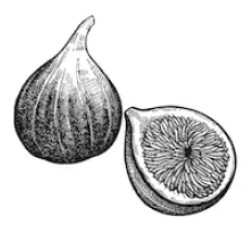
\includegraphics[width=1in,height=1.25in,clip,keepaspectratio]{fig1}}]{Michael Shell}
% Use $\backslash${\tt{begin\{IEEEbiography\}}} and then for the 1st argument use $\backslash${\tt{includegraphics}} to declare and link the author photo.
% Use the author name as the 3rd argument followed by the biography text.
% \end{IEEEbiography}

% \vspace{11pt}

% \bf{If you will not include a photo:}\vspace{-33pt}
% \begin{IEEEbiographynophoto}{John Doe}
% Use $\backslash${\tt{begin\{IEEEbiographynophoto\}}} and the author name as the argument followed by the biography text.
% \end{IEEEbiographynophoto}




\vfill

\end{document}


